\documentclass[11pt,a4paper]{article}

\usepackage[T1]{fontenc}
\usepackage{lmodern}
\usepackage[margin=1in]{geometry}
\usepackage{microtype}
\usepackage{amsmath,amssymb,amsthm,mathtools}
\usepackage{booktabs,array,multirow}
\usepackage{enumitem}
\usepackage{xcolor}
\usepackage{tikz}
\usetikzlibrary{arrows.meta,positioning,shapes.geometric,fit,backgrounds}
\usepackage{pgfplots}
\pgfplotsset{compat=1.18}
\usepackage[
  colorlinks=true,
  linkcolor=blue!55!black,
  citecolor=teal!60!black,
  urlcolor=blue!55!black
]{hyperref}
\usepackage[nameinlink,noabbrev]{cleveref}

% Theorem environments:
% Main results in Section 1 use global numbers (Theorem 1..4, Corollary 1..2).
% Internal lemmas, propositions, definitions, and theorems use section numbering.
\theoremstyle{plain}
\newtheorem{maintheorem}{Theorem}
\newtheorem{maincorollary}{Corollary}
\newtheorem{lemma}{Lemma}[section]
\newtheorem{proposition}[lemma]{Proposition}
\newtheorem{subtheorem}[lemma]{Theorem}
\newtheorem{corollary}[lemma]{Corollary}

\theoremstyle{definition}
\newtheorem{definition}[lemma]{Definition}
\newtheorem{example}[lemma]{Example}
\newtheorem{openproblem}{Open Problem}

\theoremstyle{remark}
\newtheorem{remark}[lemma]{Remark}

\crefname{maintheorem}{Theorem}{Theorems}
\crefname{maincorollary}{Corollary}{Corollaries}
\crefname{subtheorem}{Theorem}{Theorems}
\crefname{lemma}{Lemma}{Lemmas}
\crefname{proposition}{Proposition}{Propositions}
\crefname{definition}{Definition}{Definitions}
\crefname{remark}{Remark}{Remarks}
\crefname{openproblem}{Open Problem}{Open Problems}

% Mathematical macros
\newcommand{\C}{\mathbb{C}}
\newcommand{\R}{\mathbb{R}}
\newcommand{\Q}{\mathbb{Q}}
\newcommand{\Z}{\mathbb{Z}}
\newcommand{\N}{\mathbb{N}}
\newcommand{\F}{\mathbb{F}}
\newcommand{\CP}{\mathbb{CP}}
\newcommand{\Pauli}{\mathcal{P}}
\newcommand{\Zi}{\mathbb{Z}[i]}
\newcommand{\Uone}{U(1)}
\newcommand{\GL}{\mathrm{GL}}
\newcommand{\Tr}{\operatorname{Tr}}
\newcommand{\RePart}{\operatorname{Re}}
\newcommand{\ImPart}{\operatorname{Im}}
\newcommand{\supp}{\operatorname{supp}}
\newcommand{\spanF}{\operatorname{span}}
\newcommand{\imOp}{\operatorname{im}}
\newcommand{\ket}[1]{|#1\rangle}
\newcommand{\bra}[1]{\langle#1|}
\newcommand{\braket}[2]{\langle#1|#2\rangle}
\newcommand{\ketbra}[2]{|#1\rangle\langle#2|}
\newcommand{\expval}[2]{\langle#1|#2|#1\rangle}
\newcommand{\abs}[1]{\lvert#1\rvert}
\newcommand{\norm}[1]{\lVert#1\rVert}
\newcommand{\indic}[1]{\mathbf{1}_{#1}}
\newcommand{\lean}[1]{\texttt{\small #1}}
\newcommand{\leantab}[1]{\texttt{\scriptsize #1}}
\newcommand{\repoURL}{\url{https://github.com/LingyeNBird/multi-qubit-mub-nonexistence}}

\numberwithin{equation}{section}

\title{\bfseries Non-Existence of Multi-Qubit Pauli-Covariant MUB Fiducial States and Alltop Functions on \texorpdfstring{$\F_2^n$}{F2\^{}n}}
\author{LingyeNBird\thanks{Formalized Lean~4 verification code and companion scripts are publicly available at \repoURL.}}
\date{\today}

\begin{document}
\maketitle

\begin{abstract}
We prove that for every integer $n \ge 3$, no $n$-qubit pure state $\ket{\psi} \in (\C^2)^{\otimes n}$ generates a complete set of $2^n$ pairwise mutually unbiased orthonormal bases (MUBs) under the action of the $n$-qubit Pauli (product Weyl--Heisenberg) group $\Pauli_n$. This resolves---without phase-alphabet or equimodularity assumptions---Conjecture~1 and the unrestricted product-WH MUB conjecture of Damski et~al.~\cite{damski2026product}, establishes the MUB counterpart to the Godsil--Roy obstruction for product Weyl--Heisenberg SICs~\cite{godsil2009equiangular}, and refutes the product WH-MUB mechanism conjectured by Liu, Low, and Yin~\cite{liu2026maximal} (Open Quantum Problem~E28~\cite{oqpE28}) to maximize the order-$2$ stabilizer R\'enyi entropy for all $n \ge 4$.

Our proof combines three self-contained ingredients. First, for every odd $n \ge 3$, a short argument from state purity $\rho^2 = \rho$ and the irrationality of $\sqrt{2}$ rules out even the weaker two-valued condition $\abs{\expval{\psi}{P}}^2 \in \{0, 2^{-n}\}$ ($P \neq I$), with no basis-partition hypothesis. Second, for arbitrary $n$, a matrix-free symplectic reduction maps any Pauli-covariant MUB fiducial to a unimodular \emph{Alltop function} $\phi : \F_2^n \to \Uone$ whose nontrivial multiplicative derivatives all have flat Walsh--Hadamard spectra. Third, we prove that no Alltop function exists on $\F_2^n$ for any $n \ge 3$ (sharp against $n \in \{1, 2\}$): spectral quantization forces $g_a(x) \in \{(\pm 1 \pm i)/\sqrt{2}\}$ for odd $n$ (violating a triangle identity) and $g_a(x) \in \{\pm 1, \pm i\}$ for even $n = 2k \ge 4$, where a new \emph{$2$-adic affine subspace induction} in $\Zi$ via exact M\"obius inversion yields a divisibility contradiction. Consequently, every phase function on $\F_2^n$ ($n \ge 3$) obeys the strict Gowers $U^3$ bound $2^n\norm{\phi}_{U^3(\F_2^n)}^8 > 2 - 2^{-n}$.

Finally, we analyze a one-parameter spike-plus-uniform family invariant under $\GL(n,\F_2)$ and the antiunitary involution $H^{\otimes n}\circ K$, deriving an exact closed-form Pauli fourth moment $F_n(s)$ that unifies the $1$-qubit $\ket{T}$ state ($F_1 = 4/3$), the $2$-qubit MUB fiducial ($F_2 = 7/4$), and the $3$-qubit Hoggar SIC ($F_3 = 16/9$), and certifies a $4$-qubit unit state with $F_4 < 2.150521$ ($F_4(s^*) \approx 2.150520$). Every theorem in this paper is machine-verified in Lean~4 (\texttt{v4.36.0}) using only standard axioms, with zero \texttt{sorry} and zero \texttt{native\_decide}.
\end{abstract}

\tableofcontents

% ==============================================================================
\section{Introduction}\label{sec:intro}
% ==============================================================================

\subsection{Motivation and context}

Highly symmetric ensembles of pure quantum states generated as orbits of a single \emph{fiducial vector} $\ket{\psi} \in \C^d$ under a finite projective unitary group play a central role in quantum state tomography, quantum cryptography, combinatorial design theory, and the resource theory of non-stabilizerness (``magic''). Two canonical archetypes are \emph{symmetric informationally complete positive operator-valued measures} (SIC-POVMs) and \emph{mutually unbiased bases} (MUBs)~\cite{ivanovic1981geometrical,wootters1989optimal,bandyopadhyay2002new,klappenecker2005mutually}.

In an $n$-qubit Hilbert space $(\C^2)^{\otimes n} \cong \C^{\F_2^n}$ of dimension $d = 2^n$, the natural displacement group is the $n$-qubit Pauli group $\Pauli_n$, i.e., the $n$-fold tensor product of the single-qubit Weyl--Heisenberg group, indexed up to global phases by phase space $\F_2^{2n} = \F_2^n \times \F_2^n$. A celebrated theorem of Godsil and Roy~\cite{godsil2009equiangular} establishes a rigid obstruction for product Weyl--Heisenberg (WH) SICs: a pure $n$-qubit state $\ket{\psi}$ whose Pauli orbit $\{P_p\ket{\psi}\}_{p \in \F_2^{2n}}$ forms $4^n$ equiangular lines ($\abs{\expval{\psi}{P_p}}^2 = \frac{1}{d+1}$ for all $p \neq 0$) exists \emph{only} for $n = 1$ (the single-qubit tetrahedron / $\ket{T}$ state) and $n = 3$ (the $64$ Hoggar lines~\cite{hoggar1998lines}).

The present work resolves the exact counterpart of this question for \emph{mutually unbiased bases} generated by a single fiducial under $\Pauli_n$, along with its harmonic-analytic formulation in terms of \emph{Alltop functions}~\cite{alltop1980complex,klappenecker2004constructions} and the \emph{Gowers $U^3$ uniformity norm}~\cite{gowers2001new} on $\F_2^n$. Two recent developments in quantum information theory brought this question sharply into focus:
\begin{enumerate}[leftmargin=1.8em]
  \item \textbf{Product Weyl--Heisenberg covariant MUBs~\cite{damski2026product}.} In odd prime-power dimensions $d = p^n$ ($p \ge 3$), Damski, Bistro\'n, Ponterio, Czartowski, and \.Zyczkowski constructed fiducial states generating complete sets of $d$ pairwise MUBs under the product Weyl--Heisenberg group (using cubic Alltop phases for $p \ge 5$ and Galois rings for $p = 3$; together with the computational basis, equatorial fiducials yield a full set of $d+1$ MUBs). In the multi-qubit setting ($p = 2$), however, they observed that such constructions succeed for $n = 1, 2$ and appear to fail beyond $n = 2$. They conjectured (Conjecture~1 of~\cite{damski2026product}) that no $\omega_8$-phase state $\psi(x) = 2^{-n/2}\omega_8^{m_x}$ ($\omega_8 = e^{i\pi/4}$) generates a product-WH covariant set of MUBs for $n > 2$, and further proposed the stronger unrestricted conjecture that no multi-qubit product-WH MUB fiducial exists at all for $n > 2$.
  \item \textbf{Maximal multi-qubit magic and Open Quantum Problem~E28~\cite{leone2022stabilizer,liu2026maximal,oqpE28}.} In the resource theory of quantum magic, the order-$2$ stabilizer R\'enyi entropy (SRE)~\cite{leone2022stabilizer} of an $n$-qubit pure state $\ket{\psi}$ is defined via its Pauli fourth moment
  \begin{equation}\label{eq:Fn-M2-def}
    F_n(\ket{\psi}) := \sum_{p \in \F_2^{2n}} \abs{\expval{\psi}{P_p}}^4,
    \qquad
    M_2(\ket{\psi}) := -\ln\!\left(\frac{F_n(\ket{\psi})}{2^n}\right).
  \end{equation}
  Maximizing $M_2$ is equivalent to minimizing $F_n$. Applying the Cauchy--Schwarz inequality to the Parseval identity $\sum_{p \neq 0} \abs{\expval{\psi}{P_p}}^2 = d - 1$ gives the Welch/SIC lower bound
  \begin{equation}\label{eq:welch-bound}
    F_n(\ket{\psi}) \ge 1 + \frac{(d-1)^2}{d^2 - 1} = \frac{2d}{d+1},
  \end{equation}
  with equality if and only if $\ket{\psi}$ is a Pauli-covariant SIC fiducial (possible only for $n \in \{1, 3\}$, giving $F_1 = 4/3$ and $F_3 = 16/9$). Open Quantum Problem~E28~\cite{oqpE28} asks for the exact minimum of $F_n$ (maximum of $M_2$) when no product WH-SIC exists ($n \neq 1, 3$). For $n = 2$, Liu, Low, and Yin~\cite{liu2026maximal} discovered $480$ two-qubit WH-MUB fiducials attaining $F_2 = 7/4$ ($M_2 = \ln(16/7) \approx 0.826679$), provided strong numerical evidence that this is the global two-qubit optimum, and conjectured that WH-MUB fiducials yield the maximal magic states for all $n \neq 1, 3$ (which would achieve $F_n = 2 - 2^{-n}$ and $M_2 = \ln\frac{4^n}{2^{n+1}-1}$).
\end{enumerate}

In this paper, we prove in complete generality that no multi-qubit Pauli-covariant MUB fiducial exists for any $n \ge 3$, settling both lines of inquiry decisively.

\subsection{Main results}\label{sec:main-results}

We state our four main theorems and two corollaries precisely here; formal definitions of the Pauli operators $P_p$ ($p \in \F_2^{2n}$), Alltop functions, and Pauli-covariant MUB fiducials are given in \Cref{sec:prelim}, and the exact Lean~4 identifier for each machine-verified statement is catalogued in \Cref{tab:lean-map}.

\begin{maintheorem}[Non-existence of Alltop functions on $\F_2^n$]\label{thm:no-alltop}
For every integer $n \ge 3$, there is no function $\phi : \F_2^n \to \C$ with $\abs{\phi(x)} = 1$ for all $x \in \F_2^n$ such that every nontrivial multiplicative derivative $g_a(x) := \overline{\phi(x)}\,\phi(x \oplus a)$ ($a \in \F_2^n \setminus \{0\}$) has a flat Walsh--Hadamard spectrum:
\begin{equation}\label{eq:alltop-cond}
  \left\lvert \sum_{x \in \F_2^n} (-1)^{b \cdot x}\, \overline{\phi(x)}\,\phi(x \oplus a) \right\rvert^2 = 2^n
  \qquad \forall\, a \in \F_2^n \setminus \{0\},\; \forall\, b \in \F_2^n.
\end{equation}
This threshold is sharp: for $n = 2$, $\phi_2(x_0, x_1) := i^{x_0 x_1}$ (i.e., $(1, 1, 1, i)$) is an Alltop function on $\F_2^2$ (and for $n = 1$, $\phi_1(0) = 1$, $\phi_1(1) = \omega_8$ is an Alltop function on $\F_2^1$).
\end{maintheorem}

For a phase state $\psi(x) = 2^{-n/2}\phi(x)$ with $\abs{\phi(x)} = 1$, the Pauli fourth moment coincides with the eighth power of the Gowers $U^3(\F_2^n)$ uniformity norm~\cite{gowers2001new} scaled by $2^n$:
\[
  F_n(\ket{\psi}) = \sum_{a, b \in \F_2^n} \left\lvert 2^{-n} \sum_{x \in \F_2^n} (-1)^{b \cdot x}\,\overline{\phi(x)}\,\phi(x \oplus a) \right\rvert^4 = 2^n \norm{\phi}_{U^3(\F_2^n)}^8.
\]
Parseval's identity forces $F_n(\ket{\psi}) \ge 2 - 2^{-n}$ for every phase state, with equality if and only if $\phi$ is an Alltop function. \Cref{thm:no-alltop} therefore implies a strict gap in higher-order Fourier analysis over $\F_2^n$:

\begin{maincorollary}[Strict Gowers $U^3$ lower bound]\label{cor:gowers}
For every $n \ge 3$ and every unimodular function $\phi : \F_2^n \to \Uone$,
\begin{equation}\label{eq:gowers-strict}
  2^n \norm{\phi}_{U^3(\F_2^n)}^8 > 2 - 2^{-n}.
\end{equation}
\end{maincorollary}

Our second main theorem removes all phase-state and phase-alphabet restrictions and rules out Pauli-covariant MUB fiducials across all of $\CP^{2^n-1}$:

\begin{maintheorem}[Unrestricted non-existence of Pauli-covariant MUB fiducials]\label{thm:no-pauli-mub}
For every integer $n \ge 3$, there is no unit vector $\ket{\psi} \in (\C^2)^{\otimes n}$ whose Pauli orbit $\{P_p\ket{\psi}\}_{p \in \F_2^{2n}}$ partitions into $2^n$ pairwise mutually unbiased orthonormal bases; that is, there is no map $\pi : \F_2^{2n} \to \{0, \dots, 2^n - 1\}$ satisfying
\begin{align*}
  \pi(p) = \pi(q) \text{ and } p \neq q &\implies \braket{P_p\psi}{P_q\psi} = 0, \\
  \pi(p) \neq \pi(q) &\implies \abs{\braket{P_p\psi}{P_q\psi}}^2 = 2^{-n}.
\end{align*}
This threshold is sharp: for $n = 2$, $\ket{\psi_2} = \frac{1}{2}(1, 1, 1, i)$ generates $4$ pairwise MUBs under $\Pauli_2$ (and for $n = 1$, $\ket{\psi_1} = \frac{1}{\sqrt{2}}(1, \omega_8)$ generates $2$ pairwise MUBs under $\Pauli_1$).
\end{maintheorem}

Note that \Cref{thm:no-pauli-mub} does not assume \emph{a priori} that the fibers of $\pi$ have equal cardinality $2^n$, nor that $\ket{\psi}$ is unbiased with respect to the computational basis (i.e., equatorial); as we show in \Cref{lem:lagrangian}, the fibers are automatically the $2^n$ cosets of an $n$-dimensional Lagrangian subspace $H \le \F_2^{2n}$. When $\ket{\psi}$ is equatorial, adding the computational basis yields a complete set of $2^n + 1$ MUBs. Smaller partial sets of strictly fewer than $2^n$ Pauli-covariant MUBs are outside the scope of this definition.

\begin{maincorollary}[Resolution of Conjecture~1 of~\cite{damski2026product} and refutation of WH-MUB magic maximizers~\cite{liu2026maximal}]\label{cor:damski-lly}
Let $n \ge 3$.
\begin{enumerate}[label=(\alph*),leftmargin=2em]
  \item For every exponent function $m : \F_2^n \to \N$, the $\omega_8$-phase state $\psi(x) = 2^{-n/2}\omega_8^{m(x)}$ ($\omega_8 = (1+i)/\sqrt{2}$) does not generate $2^n$ pairwise MUBs under $\Pauli_n$.
  \item In particular, for every $n \ge 4$, the product WH-MUB fiducial states conjectured by Liu, Low, and Yin~\cite{liu2026maximal} (originally for $n \neq 1, 3$) to maximize the order-$2$ stabilizer R\'enyi entropy do not exist.
\end{enumerate}
\end{maincorollary}

For odd $n \ge 3$, an even stronger statement holds without any basis-partition hypothesis whatsoever:

\begin{maintheorem}[Strong odd-$n$ two-valued obstruction]\label{thm:odd-two-valued}
For every odd integer $n = 2k + 1 \ge 3$, no unit vector $\ket{\psi} \in (\C^2)^{\otimes n}$ satisfies
\[
  \abs{\expval{\psi}{P_p}}^2 \in \{0, 2^{-n}\} \qquad \forall\, p \in \F_2^{2n} \setminus \{0\}.
\]
\end{maintheorem}

Finally, to understand extremal multi-qubit magic in the absence of both product WH-SICs and product WH-MUBs (most notably $n = 4$), we analyze an explicit one-parameter family of highly symmetric states:

\begin{maintheorem}[Unified $\GL(n,\F_2)$-invariant, $(H^{\otimes n}\circ K)$-symmetric spike family]\label{thm:spike}
Let $n \ge 1$, $d = 2^n$, and let $s \in \R$ satisfy $p := 1 - \frac{d-1}{d}s > 0$ and $v^2 := -1 + 4s - \frac{4(d-1)}{d}s^2 \ge 0$. Set $\alpha := \sqrt{p}$, $u := 2p - 1$, $v := \sqrt{v^2}$, and $\beta := \frac{u + iv}{2\alpha}$. Then
\begin{equation}\label{eq:spike-def}
  \ket{\psi_n(s)} := \alpha\ket{0} + \beta \sum_{x \in \F_2^n \setminus \{0\}} \ket{x}
\end{equation}
is a unit vector in $(\C^2)^{\otimes n}$ that is strictly invariant under computational-basis permutations in $\GL(n,\F_2)$ and invariant up to global phase under the antiunitary involution $H^{\otimes n} \circ K$ (where $K$ is entrywise complex conjugation in the computational basis). Its Pauli fourth moment is given in closed form by
\begin{equation}\label{eq:spike-poly}
  F_n(\ket{\psi_n(s)}) = 1 + (d - 1)\!\left[2(1-s)^4 + \left(\frac{d}{2} - 1\right)(1 - 2s)^4 + \frac{d}{2}\left(-1 + 4s - \frac{4(d-1)}{d}s^2\right)^2\right].
\end{equation}
In particular:
\begin{enumerate}[label=(\alph*),leftmargin=2em]
  \item At $n = 1, s = 1 - 1/\sqrt{3}$, $\ket{\psi_1(s)}$ is a $1$-qubit WH-SIC ($\ket{T}$ state) with $F_1 = 4/3$.
  \item At $n = 2, s = 1/2$, $\ket{\psi_2(s)}$ is a $2$-qubit MUB fiducial with $F_2 = 7/4$.
  \item At $n = 3, s = 2/3$, $\ket{\psi_3(s)}$ is a $3$-qubit Hoggar WH-SIC with $F_3 = 16/9$.
  \item At $n = 4$, the unique critical point $s^* \approx 0.6225432$ in the feasible interval $[2/5, 2/3]$ solves the irreducible cubic $453 s^3 - 708 s^2 + 368 s - 64 = 0$, giving $F_4(\ket{\psi_4(s^*)}) \approx 2.1505201547$ ($M_2 \approx 2.006879$). Evaluating at the nearby rational witness $s = 622543/1000000$ certifies an explicit $4$-qubit unit state with $F_4 < 2.150521$.
\end{enumerate}
\end{maintheorem}

\subsection{Positioning against prior literature}

\Cref{tab:positioning} summarizes the exact dichotomy across qubit counts $n$ and places our theorems alongside the classical results of Godsil--Roy~\cite{godsil2009equiangular}, Alltop~\cite{alltop1980complex}, Klappenecker--R\"otteler~\cite{klappenecker2004constructions}, Liu--Low--Yin~\cite{liu2026maximal}, and Damski et~al.~\cite{damski2026product}.

\begin{table}[htbp]
\centering
\caption{Existence of multi-qubit product Weyl--Heisenberg (Pauli) covariant SIC fiducials, complete $2^n$-basis MUB fiducials, and Alltop functions on $\F_2^n$, together with key Pauli fourth-moment benchmarks ($F_n$; smaller $F_n$ means larger magic $M_2 = -\ln(F_n/2^n)$).}\label{tab:positioning}
\smallskip
\small
\setlength{\tabcolsep}{4.5pt}
\renewcommand{\arraystretch}{1.18}
\begin{tabular}{@{}cccccc@{}}
\toprule
$n$ ($d$) & Prod.\ WH-SIC~\cite{godsil2009equiangular} & Prod.\ WH-MUB & Alltop on $\F_2^n$ & Welch $2d/(d+1)$ & Hyp.\ MUB $2-2^{-n}$ \\
\midrule
$1$ ($2$)  & \textbf{Yes} ($\ket{T}$) & \textbf{Yes} ($\ket{\psi_1}$) & \textbf{Yes} ($\phi_1$) & $4/3 \approx 1.3333$ & $3/2 = 1.5000$ \\
$2$ ($4$)  & No                        & \textbf{Yes} ($\ket{\psi_2}$) & \textbf{Yes} ($\phi_2$) & $8/5 = 1.6000$       & $7/4 = 1.7500$ \\
$3$ ($8$)  & \textbf{Yes} (Hoggar)     & \textbf{No} (Thms.~\ref{thm:no-pauli-mub}, \ref{thm:odd-two-valued}) & \textbf{No} (Thm.~\ref{thm:no-alltop}) & $16/9 \approx 1.7778$ & $15/8 = 1.8750$ \\
$4$ ($16$) & No                        & \textbf{No} (Thm.~\ref{thm:no-pauli-mub}) & \textbf{No} (Thm.~\ref{thm:no-alltop}) & $32/17 \approx 1.8824$ & $31/16 = 1.9375$ \\
$\ge 5$    & No                        & \textbf{No} (Thm.~\ref{thm:no-pauli-mub}) & \textbf{No} (Thm.~\ref{thm:no-alltop}) & $2d/(d+1)$ & $2 - 2^{-n}$ \\
\bottomrule
\end{tabular}
\end{table}

Two subtleties merit emphasis from the outset. First, for $n = 4$, \Cref{cor:gowers} proves the strict lower bound $F_4(\ket{\psi}) > 31/16 = 1.9375$ for all \emph{phase} (equimodular) states; for \emph{general} pure states on $\CP^{15}$, the only known analytic lower bound remains the Welch/SIC bound $32/17 \approx 1.882353 < 31/16$. Thus $31/16$ is the unreachable hypothetical WH-MUB value rather than a proved general-state floor. Second, in companion numerical experiments (independent of our Lean~4 formalization), $2{,}936$ of $3{,}000$ multi-start Riemannian optimizations on $\CP^{15}$ converged to the exact cubic point $F_4(\ket{\psi_4(s^*)}) \approx 2.1505201547 > 31/16$ ($M_2 \approx 2.006879 < \ln(256/31) \approx 2.111190$); proving global optimality of this value over all of $\CP^{15}$ remains an open problem (see \Cref{sec:open}).

\subsection{Proof architecture and why \texorpdfstring{$n \in \{1, 2\}$}{n in \{1, 2\}} escape}

\Cref{fig:proof-arch} illustrates the logical architecture of our proofs. A striking feature of the argument is how transparently each obstruction reveals the exact arithmetic reason why $n = 1$ and $n = 2$ escape:
\begin{itemize}[leftmargin=1.8em]
  \item In \Cref{thm:odd-two-valued} (odd $n = 2k+1$), the purity equation $\rho^2 = \rho$ yields $M^2 = 2\bigl(2^k(2^n - 2)\bigr)^2$ with $M \in \Z$. For $n = 1$, the factor $2^1 - 2$ vanishes, permitting both the single-qubit WH-SIC $\ket{T}$ and the equatorial MUB fiducial $\ket{\psi_1}$; for every odd $n \ge 3$, $2^n - 2 \ge 6 > 0$, contradicting the irrationality of $\sqrt{2}$.
  \item In the odd-$n$ branch of \Cref{thm:no-alltop}, quantization forces $g_a(x) \in \{(\pm 1 \pm i)/\sqrt{2}\}$ for every $a \neq 0$, which violates the triangle identity $g_a(0)\,g_{a\oplus b}(a) = g_b(0)$ as soon as two distinct nonzero shifts $a, b$ exist ($n \ge 3$); at $n = 1$, there is only one nonzero shift $a = 1$, so no triangle can be formed.
  \item In the even-$n$ branch of \Cref{thm:no-alltop} ($n = 2k$), quantization lifts $\phi$ to $\psi : \F_2^{2k} \to \{\pm 1, \pm i\} \subset \Zi$, and $2$-adic affine subspace induction produces $2^k \mid \abs{\psi'(x) - \psi'(0)}^2$. At $n = 2$ ($k = 1$), there are $2k - 2 = 0$ correlation steps and $2^1 = 2$ \emph{does} divide $\abs{i - 1}^2 = 2$, admitting $\phi_2 = (1, 1, 1, i)$. For every $k \ge 2$ ($n \ge 4$), $4 \mid \abs{\psi'(x) - \psi'(0)}^2$ collapses $\psi'(x) = \pm\psi'(0)$ for all $x$, killing the imaginary spectrum and forcing a contradiction.
\end{itemize}

\begin{figure}[htbp]
\centering
\begin{tikzpicture}[
  font=\footnotesize,
  box/.style={
    draw=blue!45!black, rounded corners=3.5pt, fill=blue!4,
    align=center, inner xsep=4.5pt, inner ysep=5pt, minimum height=1.55cm
  },
  thm/.style={
    draw=teal!60!black, thick, rounded corners=3.5pt, fill=teal!8,
    align=center, inner xsep=4.5pt, inner ysep=5pt, minimum height=1.55cm
  },
  core/.style={
    draw=purple!60!black, thick, rounded corners=3.5pt, fill=purple!6,
    align=center, inner xsep=4.5pt, inner ysep=5pt, minimum height=1.55cm
  },
  arr/.style={-{Stealth[length=6pt,width=4.5pt]}, semithick, draw=black!75}
]

% Row 1: Legend (top-left, aligned with Col L) and Spectral Quantization (top-right)
\node[draw=black!25, rounded corners=3.5pt, fill=black!2, inner xsep=6pt, inner ysep=5.5pt, text width=4.15cm, align=left, font=\footnotesize, minimum height=1.55cm] (legend) at (-5.15, 10.1) {%
  \tikz[baseline=-0.5ex]\draw[draw=blue!45!black, fill=blue!4, rounded corners=1.5pt] (0,0) rectangle (0.35,0.22);\; Tool / Reduction\\[3pt]
  \tikz[baseline=-0.5ex]\draw[draw=purple!60!black, thick, fill=purple!6, rounded corners=1.5pt] (0,0) rectangle (0.35,0.22);\; Core $2$-adic Engine\\[3pt]
  \tikz[baseline=-0.5ex]\draw[draw=teal!60!black, thick, fill=teal!8, rounded corners=1.5pt] (0,0) rectangle (0.35,0.22);\; Main Theorem / Cor.
};

\node[box, text width=6.60cm] (quant) at (2.70, 10.1) {%
  {\small\textbf{Spectral Quantization (\S\ref{sec:quant})}}\\[2pt]
  $m^2 + \ell^2 = 2^{n-2}$ ($n \ge 2$)\\
  via WHT inversion \& parity
};

% Row 2: Pauli Identities + Odd/Even Alltop branches
\node[box, text width=4.25cm] (pauli) at (-5.15, 7.2) {%
  {\small\textbf{Pauli Identities (\S\ref{sec:prelim})}}\\[2pt]
  Completeness, Parseval,\\
  Self-Duality, Purity
};

\node[box, text width=4.60cm] (oddall) at (0.05, 7.2) {%
  {\small\textbf{Odd $n = 2k{+}1 \ge 3$ (\S\ref{sec:alltop-odd})}}\\[2pt]
  $g_a(x) \in \{(\pm 1 \pm i)/\sqrt{2}\}$\\
  Triangle identity contradiction
};

\node[core, text width=4.60cm] (evenall) at (5.35, 7.2) {%
  {\small\textbf{Even $n = 2k \ge 4$ (\S\ref{sec:alltop-even}--\ref{sec:final-kill})}}\\[2pt]
  $\Zi$-M\"obius $2$-adic induction\\
  $2^k \mid \abs{\psi'(x)-\psi'(0)}^2$ ($k \ge 2$)
};

% Row 3: Theorem 3, Matrix-Free Reduction, Theorem 1
\node[thm, text width=4.25cm] (thm3) at (-5.15, 4.1) {%
  {\small\textbf{Theorem~\ref{thm:odd-two-valued} (\S\ref{sec:odd-purity})}}\\[2pt]
  No two-valued state ($n \ge 3$ odd)\\
  ($M^2 = 2b^2$; $n=1$: $2^1{-}2=0$)
};

\node[box, text width=4.60cm] (red) at (0.05, 4.1) {%
  {\small\textbf{Matrix-Free Reduction}}\\[2pt]
  (\S\ref{sec:reduction}) Lagrangian $H$, symplectic\\
  basis, joint $+1$ eigenstate $v_0$
};

\node[thm, text width=4.60cm] (thm1) at (5.35, 4.1) {%
  {\small\textbf{Theorem~\ref{thm:no-alltop} (\S\ref{sec:alltop})}}\\[2pt]
  No Alltop on $\F_2^n$ ($n \ge 3$)\\
  Sharp at $n \in \{1, 2\}$
};

% Row 4: Theorem 4, Theorem 2 (& Cor. 2), Corollary 1
\node[thm, text width=4.25cm] (thm4) at (-5.15, 0.9) {%
  {\small\textbf{Theorem~\ref{thm:spike} (\S\ref{sec:spike})}}\\[2pt]
  Spike $F_n(s)$: $\ket{T}$, MUB, Hoggar\\
  $4$-qubit bound $F_4 < 2.150521$
};

\node[thm, text width=4.60cm] (thm2) at (0.05, 0.9) {%
  {\small\textbf{Theorem~\ref{thm:no-pauli-mub} (\S\ref{sec:reduction}, \S\ref{sec:alltop})}}\\[2pt]
  No Pauli-MUB fiducial ($n \ge 3$)\\
  (\& \textbf{Cor.~\ref{cor:damski-lly}}: Damski \& E28)
};

\node[thm, text width=4.60cm] (cor1) at (5.35, 0.9) {%
  {\small\textbf{Corollary~\ref{cor:gowers} (\S\ref{sec:alltop})}}\\[2pt]
  Strict Gowers $U^3$ ($n \ge 3$):\\
  $2^n\norm{\phi}_{U^3}^8 > 2 - 2^{-n}$
};

% Arrows
\draw[arr] ([xshift=-0.8cm]quant.south) -- (oddall.north);
\draw[arr] ([xshift=0.8cm]quant.south) -- (evenall.north);
\draw[arr, rounded corners=4pt] (pauli.west) -| (-7.82, 0.9) -- (thm4.west);
\draw[arr] (pauli.south) -- (thm3.north);
\draw[arr] ([xshift=0.9cm]pauli.south) -- ([xshift=-0.9cm]red.north);
\draw[arr] ([xshift=0.9cm]oddall.south) -- ([xshift=-0.9cm]thm1.north);
\draw[arr] (evenall.south) -- (thm1.north);
\draw[arr, dashed, draw=black!60] ([xshift=0.9cm]thm3.south) -- node[pos=0.48, sloped, below=2pt, font=\footnotesize]{odd-$n$ shortcut} ([xshift=-0.9cm]thm2.north);
\draw[arr] (red.south) -- (thm2.north);
\draw[arr] ([xshift=-0.9cm]thm1.south) -- ([xshift=0.9cm]thm2.north);
\draw[arr] (thm1.south) -- (cor1.north);

\end{tikzpicture}
\caption{Logical dependency structure of the main theorems. The dashed arrow indicates that for odd $n \ge 3$, \Cref{thm:odd-two-valued} combined with \Cref{lem:lagrangian} already suffices to establish \Cref{thm:no-pauli-mub}, whereas the odd-$n$ branch of \Cref{thm:no-alltop} is still needed for Alltop non-existence and \Cref{cor:gowers}.}\label{fig:proof-arch}
\end{figure}

Every theorem, lemma, and numerical bound in \Cref{thm:no-alltop,cor:gowers,thm:no-pauli-mub,cor:damski-lly,thm:odd-two-valued,thm:spike} has been completely formalized and kernel-checked in Lean~4 (\texttt{v4.36.0})~\cite{demoura2021lean4,mathlib2020lean} across $5{,}152$ lines of self-contained code with zero \texttt{sorry}, zero \texttt{native\_decide}, and only the three standard foundational axioms (\texttt{propext}, \texttt{Classical.choice}, \texttt{Quot.sound}); see \Cref{sec:lean} for the formalization architecture and module-by-theorem mapping.

\paragraph{Organization.}
\Cref{sec:prelim} establishes notation, Walsh--Hadamard inversion, Pauli identities, and formal definitions. \Cref{sec:odd-purity} presents the short direct proof of \Cref{thm:odd-two-valued}. \Cref{sec:reduction} develops the matrix-free symplectic reduction from Pauli-covariant MUB fiducials to Alltop functions (\Cref{thm:no-pauli-mub} $\Leftarrow$ \Cref{thm:no-alltop}) and verifies sharpness for $n = 1, 2$. \Cref{sec:alltop} proves \Cref{thm:no-alltop} and \Cref{cor:gowers} via spectral quantization, the odd-$n$ triangle contradiction, and the even-$n$ $2$-adic affine subspace induction in $\Zi$. \Cref{sec:spike} studies the unified spike-plus-uniform family (\Cref{thm:spike}) and its implications for four-qubit magic. \Cref{sec:lean} summarizes the pure-kernel Lean~4 formalization, and \Cref{sec:open} discusses open problems.

% ==============================================================================
\section{Preliminaries and Pauli Identities}\label{sec:prelim}
% ==============================================================================

\subsection{Binary vector spaces and the Walsh--Hadamard transform}

Let $n \ge 1$ be an integer, $d := 2^n$, and $\F_2^n := (\Z/2\Z)^n$. We write $x \oplus y$ (or $x + y$ when unambiguous inside $\F_2^n$) for bitwise addition modulo~$2$, and $x \cdot y := \sum_{j=1}^n x_j y_j \in \F_2$ for the standard bilinear dot product. Define the integer sign character
\[
  \chi(x, y) := (-1)^{x \cdot y} \in \{-1, +1\}.
\]
The standard basis vectors of $\F_2^n$ are denoted $e_1, \dots, e_n$. For any linear subspace $U \le \F_2^n$, its orthogonal complement is $U^\perp := \{a \in \F_2^n : a \cdot u = 0 \;\forall u \in U\}$.

\begin{lemma}[Character orthogonality and WHT inversion]\label{lem:wht}
Let $R$ be a commutative ring.
\begin{enumerate}[label=(\roman*),leftmargin=2em]
  \item For every linear subspace $U \le \F_2^n$, shift $v_0 \in \F_2^n$, and $a \in \F_2^n$,
  \[
    \sum_{u \in U} \chi(v_0 \oplus u, a) = \abs{U}\,\chi(v_0, a)\,\indic{a \in U^\perp}.
  \]
  In particular, $\sum_{x \in \F_2^n} \chi(x, y) = 2^n \indic{y = 0}$.
  \item For every function $f : \F_2^n \to R$, defining $\widehat{f}(u) := \sum_{y \in \F_2^n} \chi(u, y)\, f(y)$, we have the inversion identity
  \[
    \sum_{u \in \F_2^n} \chi(u, x)\,\widehat{f}(u) = 2^n f(x) \qquad \forall\, x \in \F_2^n.
  \]
  \item For every linear subspace $W \le \F_2^n$ with $\dim_{\F_2} W \ge 2$ and every $b \in \F_2^n$:
  \begin{align*}
    \abs{\{a \in W : a \cdot b = 1\}} &\text{ is even,} \\
    \abs{\{a \in W \setminus \{0\} : a \cdot b = 0\}} &\text{ is odd.}
  \end{align*}
\end{enumerate}
\end{lemma}

\begin{proof}
(i) Since $\chi(v_0 \oplus u, a) = \chi(v_0, a)\chi(u, a)$, it suffices to treat $v_0 = 0$. If $a \in U^\perp$, every summand equals $1$. If $a \notin U^\perp$, choose $v \in U$ with $v \cdot a = 1$; translating $u \mapsto u \oplus v$ negates the sum, forcing it to vanish.

(ii) Expanding $\widehat{f}(u)$ and swapping the order of summation gives
\[
  \sum_{u \in \F_2^n} \chi(u, x)\,\widehat{f}(u) = \sum_{y \in \F_2^n} \left(\sum_{u \in \F_2^n} \chi(u, x \oplus y)\right) f(y) = 2^n f(x)
\]
by (i) with $U = \F_2^n$.

(iii) Let $W_0 := \{a \in W : a \cdot b = 0\} = \ker(a \mapsto a \cdot b\vert_W)$. By rank--nullity, $\dim W_0 \ge \dim W - 1 \ge 1$, so $\abs{W_0} = 2^{\dim W_0}$ is even and $\ge 2$. Therefore $\abs{W_0 \setminus \{0\}} = 2^{\dim W_0} - 1$ is odd, and $\abs{\{a \in W : a \cdot b = 1\}} = \abs{W} - \abs{W_0} = 2^{\dim W} - 2^{\dim W_0}$ is even.
\end{proof}

\subsection{Hermitian involutive Pauli operators and core identities}

We identify $(\C^2)^{\otimes n}$ with the space $\C^{\F_2^n}$ of complex-valued functions on $\F_2^n$, equipped with the Hermitian inner product $\braket{\phi}{\psi} := \sum_{x \in \F_2^n} \overline{\phi(x)}\,\psi(x)$. A \emph{pure state} (or \emph{unit state}) is a vector $\psi \in \C^{\F_2^n}$ satisfying $\braket{\psi}{\psi} = 1$.

For each phase-space index $p = (a, b) \in \F_2^n \times \F_2^n = \F_2^{2n}$, set
\[
  \eta(p) := \begin{cases} 1 & \text{if } a \cdot b = 0, \\ i & \text{if } a \cdot b = 1, \end{cases}
\]
and define the linear operator $P_p$ on $\C^{\F_2^n}$ (corresponding to $i^{a \cdot b} Z^b X^a$) by
\begin{equation}\label{eq:pauli-def}
  (P_{(a,b)}\psi)(x) := \eta(a, b)\,(-1)^{b \cdot x}\,\psi(x \oplus a).
\end{equation}
Equip $\F_2^{2n}$ with the non-degenerate alternating symplectic bilinear form
\[
  \omega\bigl((a, b), (c, d)\bigr) := a \cdot d + b \cdot c \in \F_2.
\]
Direct coordinate evaluation verifies the following elementary properties of $\{P_p\}$:
\begin{enumerate}[label=(\arabic*),leftmargin=2em]
  \item \textbf{Involution:} $P_p^2 = I$, because $\eta(a,b)^2 (-1)^{b \cdot a} = (-1)^{a \cdot b}(-1)^{b \cdot a} = 1$.
  \item \textbf{Hermiticity and unitarity:} $\braket{\phi}{P_p \psi} = \braket{P_p \phi}{\psi}$, since substituting $x \mapsto x \oplus a$ gives $\eta(a,b)(-1)^{b \cdot a} = \overline{\eta(a,b)}$. In particular, $P_p$ is unitary and every Pauli expectation value $\expval{\psi}{P_p}$ is real.
  \item \textbf{Composition and commutation:} For all $p = (p_1, p_2)$ and $q = (q_1, q_2)$ in $\F_2^{2n}$,
  \begin{equation}\label{eq:pauli-comp}
    P_p P_q = \gamma(p, q)\, P_{p \oplus q}, \qquad \gamma(p, q) := \eta(p)\,\eta(q)\,(-1)^{q_2 \cdot p_1}\,\overline{\eta(p \oplus q)} \in \{\pm 1, \pm i\}.
  \end{equation}
  Moreover, $\gamma(p, 0) = \gamma(0, p) = \gamma(p, p) = 1$, $\gamma(p, q) = (-1)^{\omega(p, q)}\gamma(q, p)$ (hence $P_p P_q = (-1)^{\omega(p, q)} P_q P_p$), and the real/imaginary dichotomy holds:
  \begin{equation}\label{eq:gamma-cases}
  \begin{aligned}
    \omega(p, q) = 0 &\implies \gamma(p, q) \in \{+1, -1\}, \\
    \omega(p, q) = 1 &\implies \gamma(p, q) \in \{+i, -i\} \quad (\RePart\gamma(p,q) = 0).
  \end{aligned}
  \end{equation}
  Indeed, $(p \oplus q)_1 \cdot (p \oplus q)_2 = p_1 \cdot p_2 + q_1 \cdot q_2 + \omega(p, q)$ in $\F_2$, so the number of factors of $i$ in $\eta(p)\eta(q)\overline{\eta(p \oplus q)}$ has the same parity as $\omega(p, q)$.
\end{enumerate}

The next lemma records four foundational identities, proved directly on $\C^{\F_2^n}$ without invoking matrix representations.

\begin{lemma}[Pauli completeness, Parseval, symplectic self-duality, and purity]\label{lem:pauli-identities}
For all $\psi, \phi \in \C^{\F_2^n}$:
\begin{enumerate}[label=(\roman*),leftmargin=2em]
  \item \textbf{Completeness:}
  \[
    \sum_{p \in \F_2^{2n}} \expval{\psi}{P_p}\, P_p \phi = 2^n \braket{\psi}{\phi}\,\psi.
  \]
  \item \textbf{Parseval:}
  \[
    \sum_{p \in \F_2^{2n}} \expval{\psi}{P_p}\,\expval{\phi}{P_p} = 2^n \abs{\braket{\psi}{\phi}}^2.
  \]
  In particular, for every unit state $\psi$, $\sum_{p \in \F_2^{2n}} \expval{\psi}{P_p}^2 = 2^n$.
  \item \textbf{Symplectic WHT self-duality:} For every $q \in \F_2^{2n}$,
  \[
    \sum_{p \in \F_2^{2n}} (-1)^{\omega(p, q)}\,\expval{\psi}{P_p}^2 = 2^n \expval{\psi}{P_q}^2.
  \]
  \item \textbf{Purity identity ($\rho^2 = \rho$ in the Pauli basis):} For every unit state $\psi$ and every $q \in \F_2^{2n}$,
  \[
    \sum_{p \in \F_2^{2n}} \expval{\psi}{P_p}\,\gamma(q, p)\,\expval{\psi}{P_{q \oplus p}} = 2^n \expval{\psi}{P_q}.
  \]
\end{enumerate}
\end{lemma}

\begin{proof}
(i) Evaluating the left-hand side at $x \in \F_2^n$ gives
\[
  \sum_{a, b \in \F_2^n} \left(\sum_{y \in \F_2^n} \overline{\psi(y)}\,\eta(a,b)(-1)^{b \cdot y}\,\psi(y \oplus a)\right) \eta(a,b)(-1)^{b \cdot x}\,\phi(x \oplus a).
\]
Using $\eta(a,b)^2 = (-1)^{a \cdot b}$ and swapping the sums over $b$ and $y$, the inner sum over $b$ equals $\sum_{b \in \F_2^n} (-1)^{b \cdot (x \oplus y \oplus a)} = 2^n \indic{y = x \oplus a}$ by \Cref{lem:wht}(i). Substituting $y = x \oplus a$ (hence $y \oplus a = x$) and re-indexing $z = x \oplus a$ yields
\[
  2^n \left(\sum_{z \in \F_2^n} \overline{\psi(z)}\,\phi(z)\right)\psi(x) = 2^n \braket{\psi}{\phi}\,\psi(x).
\]

(ii) Take $\braket{\phi}{\,\cdot\,}$ of both sides of (i), using $\braket{\phi}{\psi}\braket{\psi}{\phi} = \abs{\braket{\psi}{\phi}}^2$.

(iii) Substitute $\phi = P_q \psi$ into (ii). By Hermiticity, involution, and commutation, we have $\expval{P_q\psi}{P_p} = \braket{\psi}{P_q P_p P_q \psi} = (-1)^{\omega(p,q)}\expval{\psi}{P_p}$, while $\abs{\braket{\psi}{P_q\psi}}^2 = \expval{\psi}{P_q}^2$.

(iv) Set $\phi = \psi$ in (i) (so $\braket{\psi}{\psi} = 1$) and take $\braket{P_q \psi}{\,\cdot\,}$ of both sides. Using Hermiticity and \eqref{eq:pauli-comp}, $\braket{P_q \psi}{P_p \psi} = \braket{\psi}{P_q P_p \psi} = \gamma(q,p)\expval{\psi}{P_{q \oplus p}}$, while $\braket{P_q\psi}{\psi} = \expval{\psi}{P_q}$.
\end{proof}

\subsection{Core definitions}

\begin{definition}[Alltop function on $\F_2^n$]\label{def:alltop}
A function $\phi : \F_2^n \to \C$ is an \emph{Alltop function} on $\F_2^n$ if $\abs{\phi(x)} = 1$ for every $x \in \F_2^n$ and every nontrivial multiplicative derivative $g_a(x) := \overline{\phi(x)}\,\phi(x \oplus a)$ ($a \in \F_2^n \setminus \{0\}$) satisfies
\[
  \abs{\widehat{g_a}(b)}^2 = \left\lvert \sum_{x \in \F_2^n} (-1)^{b \cdot x}\,\overline{\phi(x)}\,\phi(x \oplus a) \right\rvert^2 = 2^n \qquad \forall\, b \in \F_2^n.
\]
\end{definition}

\begin{definition}[Pauli-covariant MUB fiducial state]\label{def:pauli-mub}
A unit vector $\psi \in \C^{\F_2^n}$ is a \emph{Pauli-covariant MUB fiducial state} if there exists a partition map $\pi : \F_2^{2n} \to \{0, \dots, 2^n - 1\}$ such that for all $p, q \in \F_2^{2n}$:
\begin{enumerate}[label=(\roman*),leftmargin=2em]
  \item $\pi(p) = \pi(q)$ and $p \neq q \implies \braket{P_p \psi}{P_q \psi} = 0$;
  \item $\pi(p) \neq \pi(q) \implies \abs{\braket{P_p \psi}{P_q \psi}}^2 = 2^{-n}$.
\end{enumerate}
\end{definition}

\begin{remark}[Scope of \Cref{def:pauli-mub}]\label{rem:mub-scope}
\Cref{def:pauli-mub} characterizes a single fiducial vector whose Pauli orbit forms a complete family of $2^n$ pairwise mutually unbiased orthonormal bases in $(\C^2)^{\otimes n}$ (which, for equatorial states, combines with the computational basis to give a maximal set of $2^n + 1$ MUBs). Equal fiber sizes $\abs{\pi^{-1}(j)} = 2^n$ are \emph{not} assumed in \Cref{def:pauli-mub}; they are deduced automatically in \Cref{lem:lagrangian}. Smaller partial families of strictly fewer than $2^n$ pairwise MUBs inside a Pauli orbit are outside the scope of \Cref{def:pauli-mub}.
\end{remark}

\begin{remark}[Relation to the Gowers $U^3$ norm]\label{rem:gowers-u3}
Recall~\cite{gowers2001new} that for $f : \F_2^n \to \C$, the Gowers $U^3$ uniformity norm is defined by
\[
  \norm{f}_{U^3(\F_2^n)}^8 := \frac{1}{8^n} \sum_{x, h_1, h_2, h_3 \in \F_2^n} \Delta_{h_1}\Delta_{h_2}\Delta_{h_3} f(x)
  = \frac{1}{2^n} \sum_{a \in \F_2^n} \norm{g_a}_{U^2(\F_2^n)}^4,
\]
where $\Delta_h f(x) = \overline{f(x)} f(x \oplus h)$ and $g_a = \Delta_a f$. By the Plancherel identity for the $U^2$ norm, $\norm{g_a}_{U^2(\F_2^n)}^4 = 2^{-4n} \sum_{b \in \F_2^n} \abs{\widehat{g_a}(b)}^4$. Hence for a phase state $\psi(x) = 2^{-n/2}\phi(x)$ ($\abs{\phi(x)} = 1$), since $\expval{\psi}{P_{(a,b)}} = 2^{-n}\eta(a,b)\widehat{g_a}(b)$, we obtain
\begin{equation}\label{eq:Fn-U3}
  F_n(\ket{\psi}) = \sum_{a, b \in \F_2^n} \abs{\expval{\psi}{P_{(a,b)}}}^4 = \sum_{a, b \in \F_2^n} \left(\frac{\abs{\widehat{g_a}(b)}^2}{4^n}\right)^2 = 2^n \norm{\phi}_{U^3(\F_2^n)}^8.
\end{equation}
\end{remark}

% ==============================================================================
\section{Direct Purity Obstruction for Odd \texorpdfstring{$n \ge 3$}{n >= 3}}\label{sec:odd-purity}
% ==============================================================================

Before developing the general reduction to Alltop functions, we prove \Cref{thm:odd-two-valued}. Remarkably, for all odd $n \ge 3$, no basis partition or Clifford alignment is needed: state purity alone clashes with the irrationality of $\sqrt{2}$.

\begin{proof}[Proof of \Cref{thm:odd-two-valued}]
Let $n = 2k + 1 \ge 3$ ($k \ge 1$) and suppose toward a contradiction that a unit vector $\psi \in \C^{\F_2^n}$ satisfies $c_p := \expval{\psi}{P_p} \in \R$ with $c_p^2 \in \{0, 2^{-n}\}$ for every $p \neq 0$.

\emph{Step 1: Existence of a nonzero expectation.}
Since $c_0 = \braket{\psi}{\psi} = 1$ and $\sum_{p \in \F_2^{2n}} c_p^2 = 2^n \ge 8 > 1$ by \Cref{lem:pauli-identities}(ii), there exists $q \in \F_2^{2n} \setminus \{0\}$ with $c_q \neq 0$, hence $c_q^2 = 2^{-n}$.

\emph{Step 2: Real part of the purity identity.}
Take the real part of \Cref{lem:pauli-identities}(iv) at $q$ and peel off the two summands $p = 0$ and $p = q$. Since $\gamma(q, 0) = \gamma(q, q) = 1$, $c_0 = 1$, and $q \oplus q = 0$, each of these two terms contributes $c_q$, leaving
\begin{equation}\label{eq:purity-peeled}
  \sum_{p \notin \{0, q\}} \RePart\bigl(\gamma(q, p)\bigr)\, c_p\, c_{q \oplus p} = (2^n - 2)\, c_q.
\end{equation}

\emph{Step 3: Integrality and irrationality of $\sqrt{2}$.}
Multiply \eqref{eq:purity-peeled} by $2^n$. For every $p \notin \{0, q\}$, both $p \neq 0$ and $q \oplus p \neq 0$, so $c_p^2, c_{q \oplus p}^2 \in \{0, 2^{-n}\}$. Thus $(2^n c_p c_{q \oplus p})^2 \in \{0, 1\}$, which forces $2^n c_p c_{q \oplus p} \in \{-1, 0, +1\} \subset \Z$. By \eqref{eq:gamma-cases}, $\RePart\gamma(q, p) \in \{-1, 0, +1\} \subset \Z$ as well. Hence the left-hand side of $2^n \times \eqref{eq:purity-peeled}$ is an integer $M \in \Z$:
\[
  M = 2^n (2^n - 2)\, c_q.
\]
Squaring both sides and substituting $c_q^2 = 2^{-n}$ and $n = 2k + 1$ yields
\[
  M^2 = 2^n (2^n - 2)^2 = 2\bigl(2^k (2^n - 2)\bigr)^2.
\]
Since $n \ge 3$, the integer $b := 2^k(2^n - 2)$ is strictly positive. By elementary infinite descent ($a^2 = 2b^2 \Rightarrow 2 \mid a \Rightarrow 2 \mid b \Rightarrow (a/2)^2 = 2(b/2)^2$), the equation $M^2 = 2b^2$ has no integer solution with $b > 0$, a contradiction.
\end{proof}

\begin{remark}[Why $n = 1$ escapes and structural role of \Cref{thm:odd-two-valued}]\label{rem:odd-shortcut}
At $n = 1$, the factor $2^1 - 2$ vanishes, so $b = 0$ and no contradiction arises; indeed both $\ket{T}$ (where $c_p^2 = 1/3$ for $p \neq 0$) and the $1$-qubit MUB fiducial $\ket{\psi_1} = \frac{1}{\sqrt{2}}(1, \omega_8)$ (where $c_Z^2 = 0$ and $c_X^2 = c_Y^2 = 1/2$) exist. Furthermore, because every Pauli-covariant MUB fiducial automatically satisfies $c_p^2 \in \{0, 2^{-n}\}$ for all $p \neq 0$ (\Cref{lem:lagrangian}), \Cref{thm:odd-two-valued} already implies \Cref{thm:no-pauli-mub} for all odd $n \ge 3$. The odd-$n$ branch of \Cref{thm:no-alltop} in \Cref{sec:alltop-odd} is still needed to rule out Alltop functions and establish the strict Gowers $U^3$ lower bound (\Cref{cor:gowers}) for odd $n \ge 3$.
\end{remark}

% ==============================================================================
\section{Matrix-Free Reduction: Pauli-MUB Fiducials to Alltop Functions}\label{sec:reduction}
% ==============================================================================

In this section we prove that for every $n \ge 1$, the existence of a Pauli-covariant MUB fiducial implies the existence of an Alltop function on $\F_2^n$---thereby reducing \Cref{thm:no-pauli-mub} to \Cref{thm:no-alltop}. Rather than diagonalizing $2^n \times 2^n$ matrices via a global Clifford unitary, we perform the entire reduction directly on $\C^{\F_2^n}$ in three elementary steps: extracting a Lagrangian zero subgroup $H$, constructing an explicit symplectic basis without induction, and building an $H$-aligned orthonormal basis from a single trace-certified joint $+1$ eigenstate.

For a subspace $H \le \F_2^{2n}$, write $H^{\perp_\omega} := \{p \in \F_2^{2n} : \omega(p, h) = 0 \;\forall h \in H\}$ for its symplectic orthogonal complement. We call $H$ \emph{Lagrangian} if $\dim_{\F_2} H = n$ and $H^{\perp_\omega} = H$.

\begin{lemma}[Lagrangian zero subgroup and coset structure]\label{lem:lagrangian}
Suppose $\psi \in \C^{\F_2^n}$ is a Pauli-covariant MUB fiducial with partition map $\pi : \F_2^{2n} \to \{0, \dots, 2^n - 1\}$. Define
\[
  H := \{p \in \F_2^{2n} : \pi(p) = \pi(0)\}.
\]
Then:
\begin{enumerate}[label=(\roman*),leftmargin=2em]
  \item $H$ is an $n$-dimensional Lagrangian subspace of $(\F_2^{2n}, \omega)$, i.e., $\dim_{\F_2} H = n$ and $H^{\perp_\omega} = H$.
  \item $\expval{\psi}{P_p} = 0$ for all $p \in H \setminus \{0\}$, and $\abs{\expval{\psi}{P_p}}^2 = 2^{-n}$ for all $p \notin H$.
  \item For all $p, q \in \F_2^{2n}$, $\pi(p) = \pi(q) \iff p \oplus q \in H$. Consequently, the fibers of $\pi$ are precisely the $2^n$ cosets $p \oplus H$, each of cardinality $2^n$.
\end{enumerate}
\end{lemma}

\begin{proof}
First note that for any $p \in \F_2^{2n}$,
\begin{equation}\label{eq:mem-H-iff}
  p \in H \iff \bigl(p = 0 \text{ or } \expval{\psi}{P_p} = 0\bigr).
\end{equation}
Indeed, if $p \in H \setminus \{0\}$, then $\pi(0) = \pi(p)$ and $0 \neq p$ give $\expval{\psi}{P_p} = \braket{P_0\psi}{P_p\psi} = 0$; conversely, if $p \notin H$, then $\pi(0) \neq \pi(p)$ forces $\abs{\expval{\psi}{P_p}}^2 = \abs{\braket{P_0\psi}{P_p\psi}}^2 = 2^{-n} > 0$, proving both \eqref{eq:mem-H-iff} and~(ii).

Next, $H$ is a linear subspace of $\F_2^{2n}$: clearly $0 \in H$, and if $p, q \in H$, then either $p = q$ (so $p \oplus q = 0 \in H$) or $p \neq q$, in which case $\pi(p) = \pi(q)$ gives
\[
  0 = \braket{P_p \psi}{P_q \psi} = \braket{\psi}{P_p P_q \psi} = \gamma(p, q)\,\expval{\psi}{P_{p \oplus q}}.
\]
Since $\abs{\gamma(p, q)} = 1$, we get $\expval{\psi}{P_{p \oplus q}} = 0$, hence $p \oplus q \in H$ by \eqref{eq:mem-H-iff}.

By Parseval's identity (\Cref{lem:pauli-identities}(ii)) and~(ii),
\[
  2^n = \sum_{p \in \F_2^{2n}} \expval{\psi}{P_p}^2 = 1 + (4^n - \abs{H})\,2^{-n},
\]
which rearranges to $\abs{H} = 2^n$, hence $\dim_{\F_2} H = n$.

To show $H^{\perp_\omega} = H$, sum the symplectic self-duality identity (\Cref{lem:pauli-identities}(iii)) over all $q \in H$:
\[
  \sum_{p \in \F_2^{2n}} \left(\sum_{q \in H} (-1)^{\omega(p, q)}\right) \expval{\psi}{P_p}^2 = 2^n \sum_{q \in H} \expval{\psi}{P_q}^2.
\]
By symplectic character orthogonality (proved identically to \Cref{lem:wht}(i)), $\sum_{q \in H} (-1)^{\omega(p, q)} = \abs{H}\,\indic{p \in H^{\perp_\omega}} = 2^n \indic{p \in H^{\perp_\omega}}$. Meanwhile, by~(ii) the right-hand side equals $2^n \cdot 1$. Dividing by $2^n$ and peeling off $p = 0$ leaves
\[
  \sum_{p \in H^{\perp_\omega} \setminus \{0\}} \expval{\psi}{P_p}^2 = 0.
\]
Since every summand is nonnegative, $\expval{\psi}{P_p} = 0$ for all $p \in H^{\perp_\omega} \setminus \{0\}$, so $H^{\perp_\omega} \subseteq H$ by \eqref{eq:mem-H-iff}. On the other hand, applying rank--nullity to $p \mapsto (h \mapsto \omega(p, h)) \in H^*$ yields $\dim_{\F_2} H^{\perp_\omega} \ge 2n - \dim_{\F_2} H = n = \dim_{\F_2} H$. Hence $H^{\perp_\omega} = H$, completing~(i).

Finally, for~(iii), let $p, q \in \F_2^{2n}$. Since $\braket{P_p\psi}{P_q\psi} = \gamma(p, q)\expval{\psi}{P_{p \oplus q}}$ and $\abs{\gamma(p,q)} = 1$: if $\pi(p) = \pi(q)$ and $p \neq q$, then $\expval{\psi}{P_{p \oplus q}} = 0$, so $p \oplus q \in H$; conversely, if $p \oplus q \in H \setminus \{0\}$, then $\abs{\braket{P_p\psi}{P_q\psi}}^2 = \abs{\expval{\psi}{P_{p \oplus q}}}^2 = 0 \neq 2^{-n}$, forcing $\pi(p) = \pi(q)$. The case $p = q$ is trivial. Thus $\pi(p) = \pi(q) \iff p \oplus q \in H$, so the fibers of $\pi$ are the $2^n$ cosets of $H$, each of size $\abs{H} = 2^n$.
\end{proof}

\begin{lemma}[Explicit induction-free symplectic basis]\label{lem:symp-basis}
Let $H \le \F_2^{2n}$ be a Lagrangian subspace with $\F_2$-basis $f_1, \dots, f_n$. Then there exist $e_1, \dots, e_n \in \F_2^{2n}$ such that for all $1 \le i, j \le n$,
\[
  \omega(f_i, f_j) = 0, \qquad \omega(e_i, e_j) = 0, \qquad \omega(e_i, f_j) = \delta_{ij}.
\]
\end{lemma}

\begin{proof}
Since $H = H^{\perp_\omega}$, $\omega(f_i, f_j) = 0$ is immediate. Consider the linear map $L : \F_2^{2n} \to \F_2^n$ defined by $L(v)_j := \omega(v, f_j)$. Its kernel is $H^{\perp_\omega} = H$ of dimension $n$, so $\dim(\imOp L) = 2n - n = n$ and $L$ is surjective. Choose $e_{0,1}, \dots, e_{0,n} \in \F_2^{2n}$ with $L(e_{0,i}) = \delta_i$, i.e., $\omega(e_{0,i}, f_j) = \delta_{ij}$. Define explicitly
\[
  e_i := e_{0, i} \oplus \sum_{j < i} \omega(e_{0, i}, e_{0, j})\, f_j.
\]
Since $\omega(f_j, f_k) = 0$, we still have $\omega(e_i, f_k) = \omega(e_{0,i}, f_k) = \delta_{ik}$. For $k < i$, bilinearity and $\omega(f_j, f_\ell) = 0$ give
\begin{align*}
  \omega(e_i, e_k)
  &= \omega(e_{0,i}, e_{0,k})
   + \sum_{j < i} \omega(e_{0,i}, e_{0,j})\,\underbrace{\omega(f_j, e_{0,k})}_{\delta_{jk}}
   + \sum_{\ell < k} \omega(e_{0,k}, e_{0,\ell})\,\underbrace{\omega(e_{0,i}, f_\ell)}_{0 \text{ as } \ell < k < i} \\
  &= \omega(e_{0,i}, e_{0,k}) + \omega(e_{0,i}, e_{0,k}) = 0.
\end{align*}
Symmetry of $\omega$ and $\omega(e_i, e_i) = 0$ yield $\omega(e_i, e_k) = 0$ for all $i, k$.
\end{proof}

\begin{lemma}[Joint $+1$ eigenstate and reduction to an Alltop function]\label{lem:mub-to-alltop}
If there exists an $n$-qubit Pauli-covariant MUB fiducial $\psi \in \C^{\F_2^n}$, then there exists an Alltop function $\phi : \F_2^n \to \Uone$.
\end{lemma}

\begin{proof}
Let $H$ be the Lagrangian zero subgroup from \Cref{lem:lagrangian}, and let $(f_1, \dots, f_n; e_1, \dots, e_n)$ be a symplectic basis from \Cref{lem:symp-basis}. Write $F_j := P_{f_j}$ and $E_i := P_{e_i}$. For any binary vector $u \in \F_2^n$, denote the ordered products
\[
  F^u := \prod_{j : u_j = 1} F_j, \qquad E^u := \prod_{i : u_i = 1} E_i.
\]
Because the $F_j$ are pairwise commuting involutions ($\omega(f_i, f_j) = 0$) and likewise the $E_i$ are pairwise commuting involutions ($\omega(e_i, e_j) = 0$), the order of factors is irrelevant, each $F^u$ and $E^u$ is unitary, and $E^a E^x = E^{x \oplus a}$ with \emph{no phase factor at all}.

\emph{Step 1: Trace-certified joint $+1$ eigenstate.}
Define the iterated projector
\[
  \Pi := \prod_{j=1}^n \frac{I + F_j}{2} = 2^{-n} \sum_{u \in \F_2^n} F^u.
\]
Since $F_j$ commutes with every $F_k$ and satisfies $F_j^2 = I$, we have $F_j \Pi = \Pi$ for every $j$. Let $\{\delta_x\}_{x \in \F_2^n}$ be the computational basis of $\C^{\F_2^n}$. By \eqref{eq:pauli-def} and \Cref{lem:wht}(i), the trace of any Pauli operator is
\[
  \sum_{x \in \F_2^n} \braket{\delta_x}{P_{(a,b)}\delta_x} = \indic{a = 0}\sum_{x \in \F_2^n} (-1)^{b \cdot x} = 2^n \indic{(a,b) = (0,0)}.
\]
By \eqref{eq:pauli-comp}, each $F^u$ equals a unit-modulus scalar times $P_{\sum_j u_j f_j}$. Since $f_1, \dots, f_n$ are linearly independent over $\F_2$, $\sum_j u_j f_j = 0 \iff u = 0$, whence
\[
  \sum_{x \in \F_2^n} \braket{\delta_x}{\Pi \delta_x} = 2^{-n} \cdot 2^n = 1 \neq 0.
\]
Therefore $\Pi \delta_{x_0} \neq 0$ for some $x_0 \in \F_2^n$. Normalizing $v_0 := \Pi \delta_{x_0} / \norm{\Pi \delta_{x_0}}$ produces a unit vector satisfying $F_j v_0 = v_0$ for all $1 \le j \le n$.

\emph{Step 2: Clifford-aligned orthonormal basis.}
For each $x \in \F_2^n$, set $v_x := E^x v_0$.
\begin{itemize}[leftmargin=1.8em]
  \item Since $\omega(f_j, e_i) = \delta_{ij}$, $F_j E_i = (-1)^{\delta_{ij}} E_i F_j$, so $F_j v_x = (-1)^{x_j} v_x$ for every $j$, and consequently $F^b v_x = (-1)^{b \cdot x} v_x$ for every $b \in \F_2^n$.
  \item For every $a, x \in \F_2^n$, $E^a v_x = E^a E^x v_0 = E^{x \oplus a} v_0 = v_{x \oplus a}$.
  \item By unitarity of $E^x$, $\braket{v_x}{v_x} = \braket{v_0}{v_0} = 1$. If $x \neq y$, choose $j$ with $x_j \neq y_j$; then unitarity of $F_j$ gives $\braket{v_x}{v_y} = \braket{F_j v_x}{F_j v_y} = -\braket{v_x}{v_y}$, so $\braket{v_x}{v_y} = 0$.
\end{itemize}
Thus $\{v_x\}_{x \in \F_2^n}$ is an orthonormal basis of $\C^{\F_2^n}$.

\emph{Step 3: Matrix-free Pauli expectation expansion.}
Let $\alpha(x) := \braket{v_x}{\psi}$, so $\psi = \sum_{x \in \F_2^n} \alpha(x)\, v_x$. Applying $F^b E^a$ term by term and re-indexing $y = x \oplus a$ (note that Hermiticity of $F^b$ or $E^a$ is not needed) gives
\[
  F^b E^a \psi = \sum_{x \in \F_2^n} \alpha(x)\, F^b v_{x \oplus a}
  = \sum_{x \in \F_2^n} (-1)^{b \cdot (x \oplus a)}\,\alpha(x)\, v_{x \oplus a}
  = \sum_{y \in \F_2^n} (-1)^{b \cdot y}\,\alpha(y \oplus a)\, v_y.
\]
Taking the inner product with $\psi = \sum_{y \in \F_2^n} \alpha(y)\, v_y$ and using orthonormality of $\{v_y\}$ yields
\begin{equation}\label{eq:FE-eval}
  c_{a,b}\,\expval{\psi}{P_{p(a,b)}} = \braket{\psi}{F^b E^a \psi}
  = \sum_{y \in \F_2^n} (-1)^{b \cdot y}\,\overline{\alpha(y)}\,\alpha(y \oplus a),
\end{equation}
where $p(a, b) := \sum_{i=1}^n a_i e_i + \sum_{j=1}^n b_j f_j$ and $c_{a,b} \in \C$ has $\abs{c_{a,b}} = 1$ (arising from \eqref{eq:pauli-comp}).

\emph{Step 4: Equimodularity and Alltop flatness.}
Because $\omega(p(a, b), f_k) = a_k$ and $H = H^{\perp_\omega}$, we have $p(a, b) \in H \iff a = 0$.
\begin{itemize}[leftmargin=1.8em]
  \item Setting $a = 0$ in \eqref{eq:FE-eval}: for $b = 0$, the sum equals $\sum_y \abs{\alpha(y)}^2 = \braket{\psi}{\psi} = 1$; for $b \neq 0$, linear independence of $f_1, \dots, f_n$ implies $p(0, b) \in H \setminus \{0\}$, so the left-hand side vanishes by \Cref{lem:lagrangian}(ii). Thus $\sum_{y \in \F_2^n} (-1)^{b \cdot y} \abs{\alpha(y)}^2 = \indic{b = 0}$ for all $b \in \F_2^n$. By WHT inversion (\Cref{lem:wht}(ii)), $\abs{\alpha(x)}^2 = 2^{-n}$ for all $x \in \F_2^n$.
  \item Define $\phi(x) := 2^{n/2}\alpha(x)$. Then $\abs{\phi(x)} = 1$ for all $x \in \F_2^n$. For every $a \in \F_2^n \setminus \{0\}$ and every $b \in \F_2^n$, we have $p(a, b) \notin H$, so $\abs{\expval{\psi}{P_{p(a,b)}}}^2 = 2^{-n}$ by \Cref{lem:lagrangian}(ii). Multiplying \eqref{eq:FE-eval} by $2^n$ and taking squared moduli gives
  \[
    \left\lvert \sum_{y \in \F_2^n} (-1)^{b \cdot y}\,\overline{\phi(y)}\,\phi(y \oplus a) \right\rvert^2
    = (2^n)^2 \cdot \abs{c_{a,b}}^2 \cdot 2^{-n} = 2^n.
  \]
\end{itemize}
Hence $\phi$ is an Alltop function on $\F_2^n$.
\end{proof}

\begin{proof}[Proof of \Cref{thm:no-pauli-mub} and \Cref{cor:damski-lly} (assuming \Cref{thm:no-alltop})]
For $n \ge 3$, \Cref{lem:mub-to-alltop} and \Cref{thm:no-alltop} immediately show that no Pauli-covariant MUB fiducial exists in $(\C^2)^{\otimes n}$. \Cref{cor:damski-lly} follows as a direct specialization to $\omega_8$-phase states and to $n \ge 4$. Sharpness at $n = 2$ (and $n = 1$) is verified next.
\end{proof}

\begin{proposition}[Sharpness for $n = 1$ and $n = 2$]\label{prop:sharpness}
\leavevmode
\begin{enumerate}[label=(\roman*),leftmargin=2em]
  \item For $n = 2$, $\phi_2(x_0, x_1) := i^{x_0 x_1}$ (i.e., $(1, 1, 1, i)$) is an Alltop function on $\F_2^2$, and $\ket{\psi_2} := \frac{1}{2}\phi_2$ is a Pauli-covariant MUB fiducial generating $4$ pairwise MUBs under $\Pauli_2$, with $F_2(\ket{\psi_2}) = 7/4$.
  \item For $n = 1$, $\phi_1(0) := 1$, $\phi_1(1) := \omega_8 = (1+i)/\sqrt{2}$ is an Alltop function on $\F_2^1$, and $\ket{\psi_1} := \frac{1}{\sqrt{2}}(1, \omega_8)$ generates $2$ pairwise MUBs under $\Pauli_1$, with $F_1(\ket{\psi_1}) = 3/2$.
\end{enumerate}
\end{proposition}

\begin{proof}
(i) For $a \in \{(0,1), (1,0), (1,1)\}$, the multiplicative derivative $g_a(x) = \overline{\phi_2(x)}\,\phi_2(x \oplus a)$ on $(00, 01, 10, 11)$ is $(1, 1, i, -i)$, $(1, i, 1, -i)$, and $(i, 1, 1, -i)$, respectively. In each case, the four Walsh--Hadamard coefficients $\widehat{g_a}(b)$ are $\pm 2$ (when $a \cdot b = 0$) and $\pm 2i$ (when $a \cdot b = 1$), so $\abs{\widehat{g_a}(b)}^2 = 4 = 2^2$. Partitioning $\Pauli_2$ by the $X$-part $\pi(a, b) := a \in \F_2^2$: if $a_1 = a_2$ and $b_1 \neq b_2$, then $\braket{P_{(a_1,b_1)}\psi_2}{P_{(a_2,b_2)}\psi_2} = \gamma \cdot \frac{1}{4}\sum_x (-1)^{(b_1 \oplus b_2)\cdot x} = 0$; if $a_1 \neq a_2$, then $\abs{\braket{P_{(a_1,b_1)}\psi_2}{P_{(a_2,b_2)}\psi_2}}^2 = \frac{1}{16}\abs{\widehat{g_{a_1\oplus a_2}}(b_1\oplus b_2)}^2 = \frac{4}{16} = \frac{1}{4}$. Thus $3$ non-identity Paulis have expectation $0$ and $12$ have squared expectation $1/4$, giving $F_2(\ket{\psi_2}) = 1 + 12 \cdot (1/4)^2 = 7/4$.

(ii) For $n = 1$ and $a = 1$, $g_1(0) = \omega_8$ and $g_1(1) = \overline{\omega_8}$, so $\widehat{g_1}(0) = \omega_8 + \overline{\omega_8} = \sqrt{2}$ and $\widehat{g_1}(1) = \omega_8 - \overline{\omega_8} = i\sqrt{2}$, both of squared modulus $2 = 2^1$. Partitioning $\Pauli_1$ by $a \in \F_2$ gives the two pairwise MUBs $\{\ket{\psi_1}, Z\ket{\psi_1}\}$ and $\{X\ket{\psi_1}, Y\ket{\psi_1}\}$ with $F_1(\ket{\psi_1}) = 1 + 0 + (1/2)^2 + (1/2)^2 = 3/2$.
\end{proof}

% ==============================================================================
\section{Spectral Quantization and Non-Existence of Alltop Functions}\label{sec:alltop}
% ==============================================================================

This section proves \Cref{thm:no-alltop} and \Cref{cor:gowers}. The argument proceeds in four stages:
\begin{enumerate}[leftmargin=1.8em]
  \item \textbf{Elementary $\Zi$ descent (\Cref{sec:gi-descent}):} We establish power-of-two sum-of-squares classification and $(1+i)$-divisibility in $\Zi$ by direct induction, avoiding unique factorization theory.
  \item \textbf{Spectral quantization (\Cref{sec:quant}):} For every $n \ge 2$, the symmetry $g_a(x \oplus a) = \overline{g_a(x)}$ separates the real and imaginary parts of $\widehat{g_a}$ onto orthogonal half-spaces, and WHT inversion quantizes $g_a(x)$ via integer solutions to $m^2 + \ell^2 = 2^{n-2}$.
  \item \textbf{Odd $n = 2k+1 \ge 3$ (\Cref{sec:alltop-odd}):} Quantization forces $g_a(x) \in \{(\pm 1 \pm i)/\sqrt{2}\}$, immediately contradicting the triangle identity $g_a(0)\,g_{a \oplus b}(a) = g_b(0)$.
  \item \textbf{Even $n = 2k \ge 4$ (\Cref{sec:alltop-even,sec:induction,sec:final-kill}):} Quantization lifts $\phi$ (up to global phase) to $\psi : \F_2^{2k} \to \{\pm 1, \pm i\} \subset \Zi$. Its WHT factors as $z_u = (1+i)^k w_u$, and after a global unit rotation $w'_u = 1 + 2\eta_u$ satisfies $2$-adic affine correlation congruences $(\star_r)$ for all $1 \le r \le 2k - 2$. Our \emph{$2$-adic affine subspace induction theorem} (\Cref{thm:subspace-induction}) bootstraps these congruences via exact $\Zi$-M\"obius inversion to prove $2^{r-1} \mid \sum_{u \in U} \eta(v_0 \oplus u)$ up to $r = 2k - 1$. An exact WHT-to-subcube identity then forces $2^k \mid \abs{\psi'(x) - \psi'(0)}^2$, which for $k \ge 2$ collapses $\psi'(x) = \pm\psi'(0)$ and contradicts the nontrivial imaginary spectrum.
\end{enumerate}

\subsection{Elementary arithmetic descent in \texorpdfstring{$\Z$}{Z} and \texorpdfstring{$\Zi$}{Z[i]}}\label{sec:gi-descent}

Let $\Zi = \{a + bi : a, b \in \Z\}$ with norm $N(a + bi) = a^2 + b^2 = \overline{z}\,z$.

\begin{lemma}[Norm-power-of-two descent]\label{lem:sq-descent}
For all $m, \ell \in \Z$ and $j \in \N$:
\begin{enumerate}[label=(\roman*),leftmargin=2em]
  \item $m^2 + \ell^2 = 2^{2j} \implies (m, \ell) \in \{(\pm 2^j, 0),\, (0, \pm 2^j)\}$.
  \item $m^2 + \ell^2 = 2^{2j+1} \implies m \in \{\pm 2^j\}$ and $\ell \in \{\pm 2^j\}$.
\end{enumerate}
\end{lemma}

\begin{proof}
Since $x^2 \equiv 0, 1 \pmod{4}$ for every $x \in \Z$, the condition $4 \mid m^2 + \ell^2$ implies that both $m$ and $\ell$ are even. Both claims follow by induction on $j$: the base cases $m^2 + \ell^2 = 1$ and $m^2 + \ell^2 = 2$ are checked by inspection, and for $j \ge 1$ writing $m = 2m'$, $\ell = 2\ell'$ divides both sides by $4$ and reduces $j \to j - 1$.
\end{proof}

\begin{lemma}[Elementary $(1+i)^k$-divisibility]\label{lem:gi-pi-descent}
For every $k \in \N$ and $z \in \Zi$, if $2^k \mid N(z)$ in $\Z$, then $(1+i)^k \mid z$ in $\Zi$.
\end{lemma}

\begin{proof}
We induct on $k$; the case $k = 0$ is trivial. For $k \ge 1$, $2 \mid N(z) = a^2 + b^2$ (with $z = a + bi$) implies $a \equiv b \pmod{2}$, so $w := \frac{a+b}{2} + \frac{b-a}{2} i \in \Zi$ satisfies $(1+i)w = z$. Since $N(z) = N(1+i)N(w) = 2 N(w)$, we obtain $2^{k-1} \mid N(w)$, and the induction hypothesis gives $(1+i)^{k-1} \mid w$, hence $(1+i)^k \mid z$.
\end{proof}

\subsection{Spectral quantization for all \texorpdfstring{$n \ge 2$}{n >= 2}}\label{sec:quant}

\begin{lemma}[Alltop spectral quantization]\label{lem:quantization}
Let $n \ge 2$ and let $\phi : \F_2^n \to \Uone$ be an Alltop function. For each $a \in \F_2^n \setminus \{0\}$, write $g_a(x) := \overline{\phi(x)}\,\phi(x \oplus a) = r_a(x) + i t_a(x)$ with $r_a(x), t_a(x) \in \R$. Then:
\begin{enumerate}[label=(\roman*),leftmargin=2em]
  \item For every $b \in \F_2^n$:
  \begin{align*}
    a \cdot b = 0 &\implies \widehat{t_a}(b) = 0 \;\text{ and }\; \widehat{r_a}(b) = \sigma_r(a, b)\sqrt{2^n}, \\
    a \cdot b = 1 &\implies \widehat{r_a}(b) = 0 \;\text{ and }\; \widehat{t_a}(b) = \sigma_t(a, b)\sqrt{2^n},
  \end{align*}
  for signs $\sigma_r(a, b), \sigma_t(a, b) \in \{-1, +1\}$.
  \item For every $x \in \F_2^n$, there exist integers $m, \ell \in \Z$ such that
  \[
    2^n r_a(x) = 2 m \sqrt{2^n}, \qquad 2^n t_a(x) = 2 \ell \sqrt{2^n}, \qquad m^2 + \ell^2 = 2^{n-2}.
  \]
\end{enumerate}
\end{lemma}

\begin{proof}
(i) Directly from the definition, $g_a(x \oplus a) = \overline{\phi(x \oplus a)}\,\phi(x) = \overline{g_a(x)}$, so $r_a(x \oplus a) = r_a(x)$ and $t_a(x \oplus a) = -t_a(x)$. Substituting $x \mapsto x \oplus a$ in $\widehat{r_a}(b) = \sum_x (-1)^{b \cdot x} r_a(x)$ and $\widehat{t_a}(b) = \sum_x (-1)^{b \cdot x} t_a(x)$ gives
\[
  \widehat{r_a}(b) = (-1)^{a \cdot b} \widehat{r_a}(b), \qquad \widehat{t_a}(b) = -(-1)^{a \cdot b} \widehat{t_a}(b).
\]
Thus $\widehat{t_a}(b) = 0$ when $a \cdot b = 0$ and $\widehat{r_a}(b) = 0$ when $a \cdot b = 1$. Since $\widehat{r_a}(b)^2 + \widehat{t_a}(b)^2 = \abs{\widehat{g_a}(b)}^2 = 2^n$, the surviving component must equal $\pm\sqrt{2^n}$.

(ii) By WHT inversion (\Cref{lem:wht}(ii)) and~(i),
\[
  2^n r_a(x) = \left(\sum_{b : a \cdot b = 0} (-1)^{b \cdot x}\sigma_r(a, b)\right)\sqrt{2^n},
  \qquad
  2^n t_a(x) = \left(\sum_{b : a \cdot b = 1} (-1)^{b \cdot x}\sigma_t(a, b)\right)\sqrt{2^n}.
\]
Because $n \ge 2$ and $a \neq 0$, both sets $\{b \in \F_2^n : a \cdot b = 0\}$ and $\{b \in \F_2^n : a \cdot b = 1\}$ have even cardinality $2^{n-1}$ (cf.\ \Cref{lem:wht}(iii)). A sum of an even number of $\pm 1$'s is even, so the two parenthesized integer sums equal $2m$ and $2\ell$ for some $m, \ell \in \Z$. Finally, $r_a(x)^2 + t_a(x)^2 = \abs{g_a(x)}^2 = 1$ yields
\[
  4(m^2 + \ell^2)\,2^n = (2^n r_a(x))^2 + (2^n t_a(x))^2 = 4^n,
\]
whence $m^2 + \ell^2 = 2^{n-2}$.
\end{proof}

\subsection{Proof of \texorpdfstring{\Cref{thm:no-alltop}}{Theorem 1} for odd \texorpdfstring{$n = 2k + 1 \ge 3$}{n = 2k + 1 >= 3}}\label{sec:alltop-odd}

\begin{proof}[Proof of \Cref{thm:no-alltop} (odd $n$)]
Let $n = 2k + 1 \ge 3$ ($k \ge 1$) and suppose $\phi : \F_2^n \to \Uone$ is an Alltop function. For any $a \neq 0$ and $x \in \F_2^n$, \Cref{lem:quantization}(ii) gives $m, \ell \in \Z$ with $m^2 + \ell^2 = 2^{2(k-1)+1}$. By \Cref{lem:sq-descent}(ii), $m, \ell \in \{\pm 2^{k-1}\}$, which implies
\[
  r_a(x)^2 = \frac{4 m^2 \cdot 2^n}{4^n} = \frac{4 \cdot 2^{2k-2}}{2^{2k+1}} = \frac{1}{2},
  \qquad
  t_a(x)^2 = \frac{4 \ell^2 \cdot 2^n}{4^n} = \frac{1}{2}.
\]
Since $n \ge 3$, the standard basis vectors $a := e_1$ and $b := e_2$ satisfy $a \neq 0$, $b \neq 0$, and $a \oplus b \neq 0$. Using $\abs{\phi(a)}^2 = 1$, they obey the triangle identity
\[
  g_a(0)\,g_{a \oplus b}(a) = \bigl(\overline{\phi(0)}\,\phi(a)\bigr)\bigl(\overline{\phi(a)}\,\phi(b)\bigr) = \overline{\phi(0)}\,\phi(b) = g_b(0).
\]
Writing $g_a(0) = x_1 + i y_1$ and $g_{a \oplus b}(a) = x_2 + i y_2$, we compute
\[
  \RePart(g_b(0))\,\ImPart(g_b(0))
  = (x_1 x_2 - y_1 y_2)(x_1 y_2 + y_1 x_2)
  = x_1 y_1 (x_2^2 - y_2^2) + x_2 y_2 (x_1^2 - y_1^2) = 0,
\]
because $x_1^2 = y_1^2 = x_2^2 = y_2^2 = 1/2$. On the other hand, $\RePart(g_b(0))^2\,\ImPart(g_b(0))^2 = \frac{1}{2}\cdot\frac{1}{2} = \frac{1}{4} \neq 0$, a contradiction.
\end{proof}

\subsection{Even \texorpdfstring{$n = 2k \ge 4$}{n = 2k >= 4}: lifting to \texorpdfstring{$\Zi$}{Z[i]} and correlation congruences \texorpdfstring{$(\star_r)$}{(*\_r)}}\label{sec:alltop-even}

For the remainder of \Cref{sec:alltop}, let $n = 2k$ with $k \ge 2$, and suppose toward a contradiction that $\phi : \F_2^{2k} \to \Uone$ is an Alltop function.

\paragraph{Step 1: Quantization into $\{\pm 1, \pm i\} \subset \Zi$.}
Replacing $\phi$ by $\phi_0(x) := \overline{\phi(0)}\,\phi(x)$ preserves the Alltop property (each $g_a$ is unchanged since $\abs{\phi(0)} = 1$) and normalizes $\phi_0(0) = 1$. For every $a \neq 0$ and $x \in \F_2^{2k}$, \Cref{lem:quantization}(ii) gives $m, \ell \in \Z$ with $m^2 + \ell^2 = 2^{2(k-1)}$. By \Cref{lem:sq-descent}(i), $(m, \ell) \in \{(\pm 2^{k-1}, 0), (0, \pm 2^{k-1})\}$, forcing $g_a(x) \in \{+1, -1, +i, -i\}$. Since $\phi_0(x) = g_x(0)$ for $x \neq 0$ and $\phi_0(0) = 1$, $\phi_0$ lifts to a function $\psi : \F_2^{2k} \to \{+1, -1, +i, -i\} \subset \Zi$.

Define the $\Zi$-valued multiplicative-derivative WHT
\[
  \hat{g}_a(b) := \sum_{x \in \F_2^{2k}} (-1)^{b \cdot x}\,\overline{\psi(x)}\,\psi(x \oplus a) \in \Zi.
\]
Clearly $\hat{g}_0(b) = 2^{2k}\indic{b = 0}$, while by \Cref{lem:quantization}(i) (with $\sqrt{2^{2k}} = 2^k$), for every $a \neq 0$ and $b \in \F_2^{2k}$,
\begin{equation}\label{eq:ghat-zi}
  \hat{g}_a(b) = \begin{cases}
    \sigma_r(a, b)\,2^k & (a \cdot b = 0), \\
    \sigma_t(a, b)\,2^k i & (a \cdot b = 1),
  \end{cases}
  \qquad \sigma_r(a, b),\, \sigma_t(a, b) \in \{-1, +1\}.
\end{equation}

\paragraph{Step 2: Convolution identity, $(1+i)^k$-descent, and parity alignment.}
Let $z_u := \sum_{x \in \F_2^{2k}} (-1)^{u \cdot x}\,\psi(x) \in \Zi$ be the WHT of $\psi$. Direct expansion and substitution $y = x \oplus a$ give the \emph{convolution identity}
\begin{align}
  \overline{z_{u \oplus b}}\, z_u
  &= \sum_{x, y \in \F_2^{2k}} (-1)^{(u \oplus b)\cdot x + u \cdot y}\,\overline{\psi(x)}\,\psi(y) \nonumber\\
  &= \sum_{a \in \F_2^{2k}} (-1)^{u \cdot a} \sum_{x \in \F_2^{2k}} (-1)^{b \cdot x}\,\overline{\psi(x)}\,\psi(x \oplus a)
  = \sum_{a \in \F_2^{2k}} (-1)^{u \cdot a}\,\hat{g}_a(b). \label{eq:conv-z}
\end{align}
Setting $b = 0$ in \eqref{eq:conv-z} and applying \eqref{eq:ghat-zi} yields
\[
  N(z_u) = \overline{z_u}\,z_u = 2^k\!\left(2^k + \sum_{a \neq 0} (-1)^{u \cdot a}\,\sigma_r(a, 0)\right).
\]
In particular, $2^k \mid N(z_u)$ in $\Z$. By \Cref{lem:gi-pi-descent}, there exists $w_u \in \Zi$ such that
\begin{equation}\label{eq:z-factor}
  z_u = (1+i)^k\, w_u \qquad \forall\, u \in \F_2^{2k}.
\end{equation}
Since $\overline{(1+i)^k}(1+i)^k = N((1+i)^k) = 2^k$, canceling $2^k$ from \eqref{eq:conv-z} produces:
\begin{align}
  N(w_u) &= 2^k + \sum_{a \neq 0} (-1)^{u \cdot a}\,\sigma_r(a, 0), \label{eq:w-norm} \\
  \overline{w_{u \oplus b}}\, w_u &= \sum_{\substack{a \neq 0 \\ a \cdot b = 0}} (-1)^{u \cdot a}\,\sigma_r(a, b)
    \;+\; i \sum_{a \cdot b = 1} (-1)^{u \cdot a}\,\sigma_t(a, b) \qquad (b \neq 0). \label{eq:w-conv}
\end{align}
From \eqref{eq:w-norm}, $N(w_u)$ is \emph{odd} for every $u$ (as $2^k$ is even and $2^{2k} - 1$ is odd). For any $u \neq v$, setting $b := u \oplus v \neq 0$ in \eqref{eq:w-conv} shows that
\[
  \RePart(\overline{w_v}\,w_u) = \RePart(w_v)\RePart(w_u) + \ImPart(w_v)\ImPart(w_u)
\]
is a sum of $2^{2k-1} - 1$ (odd) signs, hence is odd. Because $\RePart(w_u)^2 + \ImPart(w_u)^2 \equiv 1 \pmod{2}$ and $\RePart(w_v)^2 + \ImPart(w_v)^2 \equiv 1 \pmod{2}$, mod-$2$ inspection forces $\RePart(w_u) \equiv \RePart(w_v) \pmod{2}$ for all $u, v \in \F_2^{2k}$.

Choose the unit rotation $u_{\mathrm{rot}} \in \{1, -i\}$ by setting $u_{\mathrm{rot}} := 1$ if $\RePart(w_0)$ is odd and $u_{\mathrm{rot}} := -i$ if $\RePart(w_0)$ is even, and define
\[
  \psi'(x) := u_{\mathrm{rot}}\,\psi(x) \in \{+1, -1, +i, -i\},
  \qquad
  w'_u := u_{\mathrm{rot}}\,w_u \in \Zi.
\]
Then every $w'_u$ has odd real part and even imaginary part, so we can write uniquely
\begin{equation}\label{eq:wprime-eta}
  w'_u = 1 + 2\eta_u, \qquad \eta_u \in \Zi.
\end{equation}

\paragraph{Step 3: Subspace correlation congruences $(\star_r)$.}
\begin{lemma}[Subspace correlation congruences]\label{lem:corr-congr}
For every integer $1 \le r \le 2k - 2$, every $r$-dimensional linear subspace $U \le \F_2^{2k}$, and all $v_0, b \in \F_2^{2k}$,
\begin{equation*}
  2^r \;\Big|\; \sum_{u \in U} \Bigl(\overline{\eta_{v_0 \oplus u}} + \eta_{v_0 \oplus u \oplus b} + 2\,\overline{\eta_{v_0 \oplus u}}\,\eta_{v_0 \oplus u \oplus b}\Bigr)
  \qquad \text{in } \Zi. \tag{$\star_r$}\label{eq:corr-congr}
\end{equation*}
\end{lemma}

\begin{proof}
Since $\dim U = r \le 2k - 2$, rank--nullity gives $\dim U^\perp \ge 2k - r \ge 2$. We first evaluate $S := \sum_{u \in U} \overline{w_{v_0 \oplus u \oplus b}}\,w_{v_0 \oplus u}$ using \eqref{eq:w-norm}--\eqref{eq:w-conv} and affine character orthogonality (\Cref{lem:wht}(i), $\sum_{u \in U} (-1)^{(v_0 \oplus u)\cdot a} = 2^r (-1)^{v_0 \cdot a}\indic{a \in U^\perp}$):
\begin{itemize}[leftmargin=1.8em]
  \item If $b = 0$:
  \[
    S = 2^{r+k} + 2^r \sum_{a \in U^\perp \setminus \{0\}} (-1)^{v_0 \cdot a}\,\sigma_r(a, 0).
  \]
  Since $k \ge 1$ and $\abs{U^\perp \setminus \{0\}} = 2^{\dim U^\perp} - 1$ is odd, the sum of signs is odd, so $S = 2^r \cdot (\text{odd integer}) \equiv 2^r \pmod{2^{r+1}}$ in $\Zi$.
  \item If $b \neq 0$:
  \[
    S = 2^r \sum_{\substack{a \in U^\perp \setminus \{0\} \\ a \cdot b = 0}} (-1)^{v_0 \cdot a}\,\sigma_r(a, b)
      \;+\; i \cdot 2^r \sum_{\substack{a \in U^\perp \\ a \cdot b = 1}} (-1)^{v_0 \cdot a}\,\sigma_t(a, b).
  \]
  By \Cref{lem:wht}(iii) applied to $W = U^\perp$ ($\dim U^\perp \ge 2$), the first index set has odd cardinality while the second has even cardinality. Hence $S = 2^r(A + iB)$ with $A$ odd and $B$ even, so again $S \equiv 2^r \pmod{2^{r+1}}$ in $\Zi$.
\end{itemize}
Taking complex conjugates preserves this congruence, because $\overline{2^r(A + iB)} = 2^r(A - iB)$ still has $A$ odd and $-B$ even, whence $\overline{S} \equiv 2^r \pmod{2^{r+1}}$. Moreover, since $\overline{u_{\mathrm{rot}}}\,u_{\mathrm{rot}} = 1$, we have $\overline{w'_x}\,w'_y = \overline{w_x}\,w_y$, so
\[
  \sum_{u \in U} \overline{w'_{v_0 \oplus u}}\,w'_{v_0 \oplus u \oplus b} = \overline{S} \equiv 2^r \pmod{2^{r+1}} \qquad \text{in } \Zi.
\]
Substituting $w'_x = 1 + 2\eta_x$ yields
\[
  \sum_{u \in U} \overline{w'_{v_0 \oplus u}}\,w'_{v_0 \oplus u \oplus b} - 2^r
  = 2 \sum_{u \in U} \Bigl(\overline{\eta_{v_0 \oplus u}} + \eta_{v_0 \oplus u \oplus b} + 2\,\overline{\eta_{v_0 \oplus u}}\,\eta_{v_0 \oplus u \oplus b}\Bigr),
\]
and dividing the congruence $2^{r+1} \mid (\text{LHS})$ by $2$ in $\Zi$ establishes \eqref{eq:corr-congr}.
\end{proof}

\subsection{The \texorpdfstring{$2$}{2}-adic affine subspace induction theorem}\label{sec:induction}

The heart of our even-$n$ proof is a purely algebraic bootstrap in $\Zi$ that converts the quadratic correlation congruences $(\star_r)$ into linear $2$-adic divisibilities on affine subspace sums of increasing dimension. To appreciate the mechanism before reading the details: if we expand the bilinear term $\sum_u \overline{f(u)}\,h(u, 1)$ on an $(m+1)$-dimensional subspace split into two $m$-dimensional halves $f(u) = h(u,0)$ and $h(u,1) = f(u) + \delta(u)$, the self-term $\sum_u \abs{f(u)}^2$ is already controlled by $(\star_m)$ at shift $b = 0$, while the cross-term $\sum_u \overline{f(u)}\,\delta(u)$ gains an extra factor of $2$ in its $\Zi$-M\"obius expansion precisely because $\delta(u)$ is a \emph{difference} across the $(m+1)$-st coordinate, whose M\"obius coefficients for $\abs{T} < m$ express as combinations of $(r+1)$- and $r$-dimensional subspaces in $\F_2^{m+1}$.

\begin{definition}[Subspace valuation property]\label{def:subspace-val}
For $m \in \N$, we say that $\eta : \F_2^n \to \Zi$ satisfies $(IH_m)$ if for every integer $1 \le r \le m$, every $r$-dimensional linear subspace $U \le \F_2^n$, and every shift $v_0 \in \F_2^n$,
\begin{equation*}
  2^{r-1} \;\Big|\; \sum_{u \in U} \eta(v_0 \oplus u) \qquad \text{in } \Zi. \tag{$IH_m$}\label{eq:IHm}
\end{equation*}
\end{definition}

Note that in $\Zi$, divisibility by $2^t$ holds if and only if $2^t$ divides both the real and imaginary parts in $\Z$, and therefore $2^t \mid z \iff 2^t \mid \overline{z}$.

We first record the exact $\Zi$-M\"obius inversion on $\F_2^m$. Write $[m] := \{1, \dots, m\}$, $\supp(u) := \{i \in [m] : u_i = 1\}$, and $u^S := \prod_{i \in S} u_i \in \{0, 1\} \subset \Zi$ (the indicator of $S \subseteq \supp(u)$). Notice $u^S u^T = u^{S \cup T}$ and $\sum_{u \in \F_2^m} u^S = 2^{m - \abs{S}}$.

\begin{lemma}[Exact $\Zi$-M\"obius inversion]\label{lem:mobius}
Every function $g : \F_2^m \to \Zi$ admits the exact representation
\begin{equation}\label{eq:mobius-inv}
  g(u) = \sum_{S \subseteq [m]} c_S(g)\, u^S,
  \qquad
  c_S(g) := \sum_{\supp(v) \subseteq S} (-1)^{\abs{S} - \abs{\supp(v)}}\, g(v).
\end{equation}
\end{lemma}

\begin{proof}
Substituting $c_S(g)$ into the right-hand side and swapping the sums over $S$ and $v$ gives
\[
  \sum_{v : \supp(v) \subseteq \supp(u)} g(v) \sum_{\supp(v) \subseteq S \subseteq \supp(u)} (-1)^{\abs{S} - \abs{\supp(v)}}.
\]
Setting $A := S \setminus \supp(v) \subseteq R := \supp(u) \setminus \supp(v)$, the inner sum is $\sum_{A \subseteq R} (-1)^{\abs{A}} = (1 - 1)^{\abs{R}} = \indic{R = \emptyset} = \indic{v = u}$.
\end{proof}

\begin{lemma}[$2$-adic valuation of M\"obius coefficients]\label{lem:mobius-val}
Let $m \ge 1$.
\begin{enumerate}[label=(\roman*),leftmargin=2em]
  \item If $f : \F_2^m \to \Zi$ satisfies $(IH_m)$, then for every nonempty $S \subseteq [m]$,
  \[
    2^{\abs{S} - 1} \;\big|\; c_S(f) \qquad \text{in } \Zi.
  \]
  \item Let $h : \F_2^{m+1} \to \Zi$ satisfy $(IH_m)$, and define $\delta : \F_2^m \to \Zi$ by $\delta(u) := h(u, 1) - h(u, 0)$. Then for every nonempty $T \subseteq [m]$:
  \[
    \begin{cases}
      2^{\abs{T}} \;\big|\; c_T(\delta) & \text{if } 1 \le \abs{T} \le m - 1, \\[4pt]
      2^{m-1} \;\big|\; c_T(\delta) & \text{if } \abs{T} = m.
    \end{cases}
  \]
\end{enumerate}
\end{lemma}

\begin{proof}
(i) Let $r := \abs{S} \ge 1$. If $r = 1$, $2^0 = 1$ divides everything. Suppose $2 \le r \le m$, and define the linear subspaces of $\F_2^m$
\[
  C_S := \{v \in \F_2^m : \supp(v) \subseteq S\}, \qquad
  H_S := \Bigl\{v \in C_S : \sum_{i \in S} v_i = 0 \text{ in } \F_2\Bigr\}.
\]
Clearly $\dim C_S = r$ and $\dim H_S = r - 1 \ge 1$. For $v \in C_S$, $\abs{\supp(v)}$ is even if and only if $v \in H_S$, so $(-1)^{\abs{\supp(v)}} = 2\indic{v \in H_S} - 1$. Using $(-1)^{r - \abs{\supp(v)}} = (-1)^r (-1)^{\abs{\supp(v)}}$, we obtain the exact identity
\[
  c_S(f) = (-1)^r \left(2 \sum_{v \in H_S} f(v) - \sum_{v \in C_S} f(v)\right).
\]
By $(IH_m)$, $2^{r-2} \mid \sum_{H_S} f$ (so $2^{r-1} \mid 2\sum_{H_S} f$) and $2^{r-1} \mid \sum_{C_S} f$. Thus $2^{r-1} \mid c_S(f)$.

(ii) Let $r := \abs{T} \ge 1$.
\begin{itemize}[leftmargin=1.8em]
  \item \emph{Case $1 \le r \le m - 1$.} Define the linear subspaces of $\F_2^{m+1}$
  \[
    \widetilde{C}_T := \{(u, t) \in \F_2^m \times \F_2 : \supp(u) \subseteq T\}, \qquad
    D_T := \Bigl\{(u, t) \in \widetilde{C}_T : \sum_{i \in T} u_i + t = 0 \text{ in } \F_2\Bigr\}.
  \]
  We have $\dim \widetilde{C}_T = r + 1 \le m$ and $\dim D_T = r \le m - 1$. For each $u$ with $\supp(u) \subseteq T$, the pair $(u, 0)$ lies in $D_T$ if $\abs{\supp(u)}$ is even, while $(u, 1)$ lies in $D_T$ if $\abs{\supp(u)}$ is odd. Consequently,
  \[
    \bigl(h(u, 0) + h(u, 1)\bigr) - 2\,h\bigl(u, \abs{\supp(u)} \bmod 2\bigr)
    = (-1)^{\abs{\supp(u)}}\bigl(h(u, 1) - h(u, 0)\bigr).
  \]
  Summing over $\supp(u) \subseteq T$ and multiplying by $(-1)^r$ yields the exact identity
  \[
    c_T(\delta) = (-1)^r \left(\sum_{w \in \widetilde{C}_T} h(w) - 2 \sum_{w \in D_T} h(w)\right).
  \]
  Since $1 \le r < r + 1 \le m$, applying $(IH_m)$ to $h$ gives $2^r \mid \sum_{\widetilde{C}_T} h$ and $2^{r-1} \mid \sum_{D_T} h$ (hence $2^r \mid 2\sum_{D_T} h$). Therefore $2^r \mid c_T(\delta)$.
  \item \emph{Case $r = m$.} Because $(IH_m)$ holds for \emph{every} affine subspace of $\F_2^{m+1}$ of dimension $\le m$ (not only linear subspaces through $0$), both slices $f_0(u) := h(u, 0)$ and $f_1(u) := h(u, 1) = h((0,1) \oplus (u,0))$ inherit $(IH_m)$ on $\F_2^m$. Applying part~(i) to both $f_1$ and $f_0$ shows $2^{m-1} \mid c_T(f_1)$ and $2^{m-1} \mid c_T(f_0)$, whence $2^{m-1} \mid c_T(\delta) = c_T(f_1) - c_T(f_0)$. \qedhere
\end{itemize}
\end{proof}

\begin{lemma}[Product-difference valuation]\label{lem:prod-diff}
Let $m \ge 1$ and let $h : \F_2^{m+1} \to \Zi$ satisfy $(IH_m)$. Setting $f(u) := h(u, 0)$ and $\delta(u) := h(u, 1) - h(u, 0)$, we have
\[
  2^{m-1} \;\Big|\; \sum_{u \in \F_2^m} \overline{f(u)}\,\delta(u) \qquad \text{in } \Zi.
\]
\end{lemma}

\begin{proof}
Expanding $\overline{f(u)} = \sum_S \overline{c_S(f)}\,u^S$ and $\delta(u) = \sum_T c_T(\delta)\,u^T$ via \Cref{lem:mobius} and using $\sum_{u \in \F_2^m} u^S u^T = \sum_{u \in \F_2^m} u^{S \cup T} = 2^{m - \abs{S \cup T}}$, we obtain
\[
  \sum_{u \in \F_2^m} \overline{f(u)}\,\delta(u)
  = \sum_{S, T \subseteq [m]} \overline{c_S(f)}\,c_T(\delta)\,2^{m - \abs{S \cup T}}.
\]
Note that $f$ satisfies $(IH_m)$ on $\F_2^m$, so \Cref{lem:mobius-val}(i) and conjugation invariance of $2$-adic divisibility give $2^{\abs{S}-1} \mid \overline{c_S(f)}$ whenever $S \neq \emptyset$. We verify that every $(S, T)$-summand is divisible by $2^{m-1}$:
\begin{itemize}[leftmargin=1.8em]
  \item $T = \emptyset$, $S = \emptyset$: the factor $2^{m - 0} = 2^m$ is divisible by $2^{m-1}$.
  \item $T = \emptyset$, $\abs{S} \ge 1$: $\overline{c_S(f)}\,2^{m - \abs{S}}$ is divisible by $2^{(\abs{S}-1) + (m - \abs{S})} = 2^{m-1}$.
  \item $1 \le \abs{T} \le m - 1$: by \Cref{lem:mobius-val}(ii), $2^{\abs{T}} \mid c_T(\delta)$. If $S = \emptyset$, then $c_T(\delta)\,2^{m - \abs{T}}$ is divisible by $2^m$; if $\abs{S} \ge 1$, then $\overline{c_S(f)}\,c_T(\delta)\,2^{m - \abs{S \cup T}}$ is divisible by $2^{(\abs{S}-1) + \abs{T} + (m - \abs{S \cup T})}$, and $(\abs{S}-1) + \abs{T} + (m - \abs{S \cup T}) \ge m - 1$ since $\abs{S} + \abs{T} \ge \abs{S \cup T}$.
  \item $\abs{T} = m$: by \Cref{lem:mobius-val}(ii), $2^{m-1} \mid c_T(\delta)$ directly. \qedhere
\end{itemize}
\end{proof}

We now assemble the full induction.

\begin{subtheorem}[$2$-adic affine subspace induction]\label{thm:subspace-induction}
Let $M \ge 0$ and let $\eta : \F_2^n \to \Zi$ satisfy the correlation congruence \eqref{eq:corr-congr} for every integer $1 \le r \le M$. Then $\eta$ satisfies $(IH_{M+1})$.
\end{subtheorem}

\begin{proof}
We induct on $M$. For $M = 0$, $(IH_1)$ requires $2^{1-1} = 1 \mid \sum_{u \in U} \eta(v_0 \oplus u)$, which is trivial.

For the induction step, assume $m \ge 1$, $(IH_m)$ holds for $\eta$, and $(\star_m)$ holds for $\eta$. To prove $(IH_{m+1})$, let $W \le \F_2^n$ be an $(m+1)$-dimensional subspace and $v_0 \in \F_2^n$. Pick an $\F_2$-basis $b_1, \dots, b_{m+1}$ of $W$, set $V := \spanF_{\F_2}(b_1, \dots, b_m)$ ($\dim V = m$) and $b := b_{m+1}$, and pull back $\eta$ along the injective affine map $\Phi(x_1, \dots, x_{m+1}) := v_0 \oplus \sum_{j=1}^{m+1} x_j b_j$ by defining $h(w) := \eta(\Phi(w))$ on $\F_2^{m+1}$. Because $\Phi$ maps every $r$-dimensional affine subspace of $\F_2^{m+1}$ bijectively onto an $r$-dimensional affine subspace of $\F_2^n$, $h$ inherits $(IH_m)$ on $\F_2^{m+1}$. Writing $f(u) := h(u, 0)$ and $\delta(u) := h(u, 1) - f(u)$ on $\F_2^m$, we have
\[
  \sum_{w \in W} \eta(v_0 \oplus w) = \sum_{u \in \F_2^m} \bigl(f(u) + h(u, 1)\bigr).
\]
We proceed in three short steps:
\begin{enumerate}[leftmargin=1.8em]
  \item \emph{Norm cancellation at shift $0$.} Applying $(\star_m)$ on $V$ with shift $0$ gives
  \[
    2^m \;\Big|\; \sum_{u \in \F_2^m} \bigl(\overline{f(u)} + f(u) + 2\abs{f(u)}^2\bigr).
  \]
  By $(IH_m)$ on $V$, $2^{m-1} \mid \sum_u f(u)$, hence $2^m \mid 2\RePart\sum_u f(u) = \sum_u (\overline{f(u)} + f(u))$. Subtracting yields $2^m \mid 2\sum_u \abs{f(u)}^2$.
  \item \emph{Cross-product elimination.} By \Cref{lem:prod-diff}, $2^{m-1} \mid \sum_u \overline{f(u)}\,\delta(u)$, so $2^m \mid 2\sum_u \overline{f(u)}\,\delta(u)$. Adding this to $2^m \mid 2\sum_u \abs{f(u)}^2$ gives
  \[
    2^m \;\Big|\; 2 \sum_{u \in \F_2^m} \overline{f(u)}\,h(u, 1).
  \]
  \item \emph{Real and imaginary parts at shift $b$.} Applying $(\star_m)$ on $V$ with shift $b = b_{m+1}$ gives $2^m \mid \sum_u \bigl(\overline{f(u)} + h(u, 1) + 2\overline{f(u)}h(u, 1)\bigr)$. Subtracting step~2 leaves
  \[
    2^m \;\Big|\; \sum_{u \in \F_2^m} \bigl(\overline{f(u)} + h(u, 1)\bigr) \qquad \text{in } \Zi.
  \]
  Taking the real part immediately gives $2^m \mid \sum_u \bigl(\RePart f(u) + \RePart h(u, 1)\bigr)$. Taking the imaginary part gives $2^m \mid \sum_u \bigl(\ImPart h(u, 1) - \ImPart f(u)\bigr)$; adding $2\sum_u \ImPart f(u)$ (which is divisible by $2 \cdot 2^{m-1} = 2^m$ by $(IH_m)$) gives $2^m \mid \sum_u \bigl(\ImPart f(u) + \ImPart h(u, 1)\bigr)$.
\end{enumerate}
Therefore $2^m \mid \sum_{w \in W} \eta(v_0 \oplus w)$ in $\Zi$, establishing $(IH_{m+1})$.
\end{proof}

\subsection{Final contradiction for all even \texorpdfstring{$n = 2k \ge 4$}{n = 2k >= 4}}\label{sec:final-kill}

We connect $(IH_{n-1})$ back to the Walsh--Hadamard transform via an exact subcube expansion.

\begin{lemma}[WHT-to-subcube identity and congruence]\label{lem:wht-subcube}
Let $n \ge 2$ and let $\eta : \F_2^n \to \Zi$ satisfy $(IH_{n-1})$. Then for all $x, y \in \F_2^n$,
\[
  2^n \;\Big|\; \sum_{u \in \F_2^n} (-1)^{u \cdot x}(1 + 2\eta_u) - \sum_{u \in \F_2^n} (-1)^{u \cdot y}(1 + 2\eta_u) \qquad \text{in } \Zi.
\]
\end{lemma}

\begin{proof}
Writing $(-1)^{u_i x_i} = 1 - 2 u_i x_i$ in $\Zi$ and expanding the product over $i \in [n]$ gives
\[
  (-1)^{u \cdot x} = \prod_{i=1}^n (1 - 2 u_i x_i) = \sum_{T \subseteq [n]} (-2)^{\abs{T}} x^T u^T.
\]
Multiplying by $\eta_u$ and summing over $u \in \F_2^n$ yields the exact WHT-to-subcube identity
\begin{equation}\label{eq:wht-subcube}
  \sum_{u \in \F_2^n} (-1)^{u \cdot x}\,\eta_u
  = \sum_{T \subseteq [n]} (-2)^{\abs{T}}\, x^T \sum_{u : T \subseteq \supp(u)} \eta_u.
\end{equation}
We claim that $2^n \mid \bigl(\sum_u (-1)^{u \cdot z}(1 + 2\eta_u) - 2\sum_u \eta_u\bigr)$ for every $z \in \F_2^n$; subtracting the congruences for $z = x$ and $z = y$ then proves the lemma. First, $\sum_u (-1)^{u \cdot z} = 2^n \indic{z = 0}$ is divisible by $2^n$. Second, peeling off the $T = \emptyset$ term of $2 \times \eqref{eq:wht-subcube}$ cancels $2\sum_u \eta_u$, leaving a sum over nonempty $T \subseteq [n]$ of terms
\[
  2 \cdot (-2)^{\abs{T}}\, z^T \sum_{u : T \subseteq \supp(u)} \eta_u.
\]
\begin{itemize}[leftmargin=1.8em]
  \item If $1 \le \abs{T} \le n - 1$, then $V_T := \{u \in \F_2^n : T \subseteq \supp(u)\}$ is an $(n - \abs{T})$-dimensional affine subspace of $\F_2^n$ with $1 \le n - \abs{T} \le n - 1$. By $(IH_{n-1})$, $2^{n - \abs{T} - 1} \mid \sum_{u \in V_T} \eta_u$, so multiplying by $2 \cdot (-2)^{\abs{T}}$ gives divisibility by $2 \cdot 2^{\abs{T}} \cdot 2^{n - \abs{T} - 1} = 2^n$.
  \item If $\abs{T} = n$, the prefactor $2 \cdot (-2)^n$ is already divisible by $2^n$.
\end{itemize}
Hence every summand is divisible by $2^n$, completing the proof.
\end{proof}

\begin{proof}[Proof of \Cref{thm:no-alltop} (even $n = 2k \ge 4$)]
By \Cref{lem:corr-congr}, $\eta$ satisfies $(\star_r)$ for all $1 \le r \le 2k - 2$. Applying \Cref{thm:subspace-induction} with $M = 2k - 2$ yields $(IH_{2k-1})$. Therefore \Cref{lem:wht-subcube} gives, for all $x, y \in \F_2^{2k}$,
\begin{equation}\label{eq:wht-diff-div}
  2^{2k} \;\Big|\; \sum_{u \in \F_2^{2k}} (-1)^{u \cdot x}(1 + 2\eta_u) - \sum_{u \in \F_2^{2k}} (-1)^{u \cdot y}(1 + 2\eta_u) \qquad \text{in } \Zi.
\end{equation}
On the other hand, by WHT inversion on $\psi$ (\Cref{lem:wht}(ii)), \eqref{eq:z-factor}, and the exact identity $2^{2k} = (-1)^k (1+i)^{4k}$ in $\Zi$ (since $(1+i)^4 = -4$),
\[
  (1+i)^k \sum_{u \in \F_2^{2k}} (-1)^{u \cdot x}(1 + 2\eta_u)
  = u_{\mathrm{rot}} \sum_{u \in \F_2^{2k}} (-1)^{u \cdot x} z_u
  = u_{\mathrm{rot}}\,2^{2k}\psi(x)
  = (-1)^k (1+i)^{4k}\,\psi'(x).
\]
Canceling the nonzero factor $(1+i)^k$ in the integral domain $\Zi$ gives
\[
  \sum_{u \in \F_2^{2k}} (-1)^{u \cdot x}(1 + 2\eta_u) = (-1)^k (1+i)^{3k}\,\psi'(x).
\]
Substituting this into \eqref{eq:wht-diff-div} yields $2^{2k} \mid (-1)^k (1+i)^{3k}\bigl(\psi'(x) - \psi'(y)\bigr)$ in $\Zi$. Taking $\Zi$-norms gives
\[
  2^{4k} \;\Big|\; 2^{3k}\, N\bigl(\psi'(x) - \psi'(y)\bigr)
  \quad \Longrightarrow \quad
  2^k \;\Big|\; N\bigl(\psi'(x) - \psi'(y)\bigr) \qquad \text{in } \Z.
\]
Since $k \ge 2$, we have $4 \mid N\bigl(\psi'(x) - \psi'(0)\bigr)$ for every $x \in \F_2^{2k}$. However, $\psi'(x), \psi'(0) \in \{+1, -1, +i, -i\}$, whose pairwise squared Euclidean distances lie in $\{0, 2, 4\}$, with distance $2$ occurring precisely when one value lies in $\{\pm 1\}$ and the other in $\{\pm i\}$. Thus $4 \mid N(\psi'(x) - \psi'(0))$ forces
\[
  \psi'(x) = \pm \psi'(0) \qquad \forall\, x \in \F_2^{2k}.
\]
Now pick $a_0 := e_1 \neq 0$. For every $x \in \F_2^{2k}$,
\[
  \overline{\psi(x)}\,\psi(x \oplus a_0) = \overline{\psi'(x)}\,\psi'(x \oplus a_0) \in \{+1, -1\}
\]
is purely real, whence $\ImPart(\hat{g}_{a_0}(a_0)) = 0$. Yet $a_0 \cdot a_0 = 1$ in $\F_2$, so \eqref{eq:ghat-zi} requires $\ImPart(\hat{g}_{a_0}(a_0)) = \pm 2^k \neq 0$, a contradiction.
\end{proof}

\subsection{Proof of \texorpdfstring{\Cref{cor:gowers}}{Corollary 1} (strict Gowers \texorpdfstring{$U^3$}{U\^{}3} lower bound)}\label{sec:proof-gowers}

\begin{proof}[Proof of \Cref{cor:gowers}]
Let $n \ge 3$ and let $\phi : \F_2^n \to \Uone$. Write $c_a(b) := \abs{\widehat{g_a}(b)}^2$. At $a = 0$, $g_0 \equiv 1$, so $c_0(b) = 4^n \indic{b = 0}$, contributing $1$ to $F_n(\phi) = 2^n\norm{\phi}_{U^3(\F_2^n)}^8$ in \eqref{eq:Fn-U3}. For every $a \in \F_2^n$, Parseval's identity for the WHT of $g_a$ gives $\sum_{b \in \F_2^n} c_a(b) = 2^n \sum_{x \in \F_2^n} \abs{g_a(x)}^2 = 4^n$, from which the exact variance identity follows:
\[
  \sum_{b \in \F_2^n} \left(\frac{c_a(b)}{4^n}\right)^2
  = \frac{1}{2^n} + \frac{1}{4^{2n}} \sum_{b \in \F_2^n} \bigl(c_a(b) - 2^n\bigr)^2.
\]
Summing over all $2^n - 1$ nonzero $a \in \F_2^n \setminus \{0\}$ and adding the $a = 0$ contribution yields
\[
  2^n \norm{\phi}_{U^3(\F_2^n)}^8
  = 1 + (2^n - 1)\frac{1}{2^n} + \frac{1}{4^{2n}} \sum_{a \neq 0} \sum_{b \in \F_2^n} \bigl(c_a(b) - 2^n\bigr)^2
  = 2 - 2^{-n} + \frac{1}{4^{2n}} \sum_{a \neq 0} \sum_{b \in \F_2^n} \bigl(c_a(b) - 2^n\bigr)^2.
\]
By \Cref{thm:no-alltop}, $\phi$ is not an Alltop function, so there exist $a_0 \neq 0$ and $b_0 \in \F_2^n$ with $c_{a_0}(b_0) \neq 2^n$. The sum of squares is therefore strictly positive, giving $2^n \norm{\phi}_{U^3(\F_2^n)}^8 > 2 - 2^{-n}$.
\end{proof}

% ==============================================================================
\section{Unified Spike-Plus-Uniform Family and Four-Qubit Magic}\label{sec:spike}
% ==============================================================================

With product WH-SICs absent for $n \notin \{1, 3\}$~\cite{godsil2009equiangular} and product WH-MUB fiducials absent for all $n \ge 3$ (\Cref{thm:no-pauli-mub}), the first open dimension for Open Quantum Problem~E28~\cite{oqpE28} is $n = 4$ ($d = 16$). We now prove \Cref{thm:spike}, showing that a single one-parameter family of spike-plus-uniform states unifies the known optimal magic states across $n = 1, 2, 3$ and produces a striking candidate global extremizer at $n = 4$.

\subsection{Symmetry and exact Pauli spectrum}

Fix $n \ge 1$, $d = 2^n$, and $s \in \R$ satisfying the feasibility conditions
\begin{equation}\label{eq:spike-feasible}
  p := 1 - \frac{d-1}{d}s > 0, \qquad
  v^2 := -1 + 4s - \frac{4(d-1)}{d}s^2 \ge 0.
\end{equation}
Notice that the quadratic $-1 + 4s - \frac{4(d-1)}{d}s^2 \ge 0$ defines the closed interval
\[
  s \in \left[\frac{d - \sqrt{d}}{2(d - 1)},\; \frac{d + \sqrt{d}}{2(d - 1)}\right],
\]
on which $p > 0$ holds automatically for every $n \ge 1$. Set $\alpha := \sqrt{p} > 0$, $u := 2p - 1$, $v := \sqrt{v^2} \ge 0$, $\beta := \frac{u + iv}{2\alpha}$, and $\ket{\psi_n(s)} := \alpha\ket{0} + \beta \sum_{x \neq 0}\ket{x}$.

\begin{proof}[Proof of \Cref{thm:spike}]
\emph{Step 1: Unit norm.}
Direct expansion gives
\[
  u^2 + v^2 = \left(1 - \frac{2(d-1)}{d}s\right)^2 + \left(-1 + 4s - \frac{4(d-1)}{d}s^2\right)
  = \frac{4s}{d}\left(1 - \frac{d-1}{d}s\right) = 4p\,\frac{s}{d},
\]
so $\abs{\beta}^2 = \frac{u^2 + v^2}{4\alpha^2} = \frac{s}{d}$. Hence $\braket{\psi_n(s)}{\psi_n(s)} = \alpha^2 + (d-1)\abs{\beta}^2 = p + \frac{d-1}{d}s = 1$.

\emph{Step 2: $\GL(n, \F_2)$ invariance and antiunitary $(H^{\otimes n}\circ K)$ symmetry.}
Any invertible linear transformation $A \in \GL(n, \F_2)$ fixes $0$ and permutes $\F_2^n \setminus \{0\}$, so $\ket{\psi_n(s)}$ is strictly invariant under the corresponding computational-basis permutation $U_A\ket{x} = \ket{Ax}$.

Under the $n$-qubit Hadamard transform $(H^{\otimes n}\psi)_y = d^{-1/2}\sum_{x \in \F_2^n} (-1)^{y \cdot x}\psi(x)$, we have
\[
  (H^{\otimes n}\psi)_0 = \frac{\alpha + (d-1)\beta}{\sqrt{d}},
  \qquad
  (H^{\otimes n}\psi)_y = \frac{\alpha - \beta}{\sqrt{d}} \quad (y \neq 0),
\]
using $\sum_{x \neq 0}(-1)^{y \cdot x} = -1$ for $y \neq 0$. Moreover, using $2\alpha\RePart(\beta) = u = 2p - 1$, $\abs{\beta}^2 = s/d$, and $\alpha^2 = p$, we observe the exact identity
\[
  \bigl(\alpha + (d-1)\beta\bigr)\overline{\beta} - \alpha(\alpha - \beta)
  = 2\alpha\RePart(\beta) + (d-1)\abs{\beta}^2 - \alpha^2
  = (2p - 1) + (1 - p) - p = 0.
\]
Setting $e^{i\theta} := \frac{\alpha + (d-1)\beta}{\alpha\sqrt{d}}$ gives $(H^{\otimes n}\psi)_0 = e^{i\theta}\overline{\alpha}$ (as $\alpha \in \R$) and, dividing the identity above by $\alpha\sqrt{d}$, $(H^{\otimes n}\psi)_y = e^{i\theta}\overline{\beta}$ for all $y \neq 0$. Since $H^{\otimes n}$ is unitary and both $\ket{\psi_n(s)}$ and $\ket{\overline{\psi_n(s)}}$ are unit vectors, $\abs{e^{i\theta}} = 1$. Thus
\begin{equation}\label{eq:antiunitary-sym}
  H^{\otimes n}\ket{\psi_n(s)} = e^{i\theta}\ket{\overline{\psi_n(s)}},
\end{equation}
meaning $\ket{\psi_n(s)}$ is invariant up to global phase under the \emph{antiunitary} involution $H^{\otimes n} \circ K$. Because $H^{\otimes n} P_{(a,b)} H^{\otimes n} = (-1)^{a \cdot b} P_{(b,a)}$ and $\overline{P_{(b,a)}} = (-1)^{a \cdot b} P_{(b,a)}$ in the computational basis, the two sign factors cancel and \eqref{eq:antiunitary-sym} immediately implies exact phase-space duality
\[
  \expval{\psi_n(s)}{P_{(a,b)}} = \expval{\psi_n(s)}{P_{(b,a)}} \qquad \forall\, a, b \in \F_2^n.
\]
In particular, $\ket{\psi_n(s)}$ is \emph{not} an eigenstate of the unitary $H^{\otimes n}$ alone: direct evaluation gives $\abs{\expval{\psi_3(2/3)}{H^{\otimes 3}}} = \sqrt{2}/3 \approx 0.4714$ and $\abs{\expval{\psi_4(s^*)}{H^{\otimes 4}}} \approx 0.6691$.

\emph{Step 3: Evaluation over the five Pauli orbits.}
Using $\overline{\alpha}\beta = \frac{u + iv}{2}$, $\overline{\beta}\alpha = \frac{u - iv}{2}$, and $\abs{\beta}^2 = s/d$, direct summation yields the five orbits listed in \Cref{tab:spike-orbits}:
\begin{itemize}[leftmargin=1.8em]
  \item $(a, b) = (0, 0)$: $\expval{\psi}{I} = 1$ (count $1$).
  \item $a = 0, b \neq 0$: $\expval{\psi}{P_{(0,b)}} = \alpha^2 + \abs{\beta}^2 \sum_{x \neq 0}(-1)^{b \cdot x} = p - \frac{s}{d} = 1 - s$ (count $d - 1$).
  \item $a \neq 0, b = 0$: separating $x = 0$, $x = a$, and the remaining $d - 2$ points gives $\overline{\alpha}\beta + \overline{\beta}\alpha + (d-2)\abs{\beta}^2 = u + \frac{d-2}{d}s = 1 - s$ (count $d - 1$).
  \item $a \neq 0, b \neq 0, a \cdot b = 0$: since $(-1)^{b \cdot a} = 1$, $\sum_{x \notin \{0, a\}} (-1)^{b \cdot x} = 0 - 1 - 1 = -2$, giving $u - \frac{2s}{d} = 1 - 2s$ (count $(d-1)(d/2 - 1)$).
  \item $a \neq 0, a \cdot b = 1$: here $\eta(a,b) = i$, $(-1)^{b \cdot a} = -1$, and $\sum_{x \notin \{0,a\}} (-1)^{b \cdot x} = 0 - 1 - (-1) = 0$, giving $i(\overline{\alpha}\beta - \overline{\beta}\alpha) = i(iv) = -v$ (count $(d-1)(d/2)$).
\end{itemize}
Summing the fourth powers over the five orbits yields \eqref{eq:spike-poly}.

\begin{table}[htbp]
\centering
\caption{Exact Pauli expectation spectrum of the spike-plus-uniform state $\ket{\psi_n(s)}$ ($d = 2^n$).}\label{tab:spike-orbits}
\smallskip
\renewcommand{\arraystretch}{1.15}
\begin{tabular}{@{}lcc@{}}
\toprule
Pauli orbit $(a, b) \in \F_2^n \times \F_2^n$ & Count & $\expval{\psi_n(s)}{P_{(a,b)}}$ \\
\midrule
$a = 0,\; b = 0$ & $1$ & $1$ \\
$a = 0,\; b \neq 0$ & $d - 1$ & $1 - s$ \\
$a \neq 0,\; b = 0$ & $d - 1$ & $1 - s$ \\
$a \neq 0,\; b \neq 0,\; a \cdot b = 0$ & $(d - 1)(d/2 - 1)$ & $1 - 2s$ \\
$a \neq 0,\; a \cdot b = 1$ & $(d - 1)(d/2)$ & $-v$ \\
\bottomrule
\end{tabular}
\end{table}

\emph{Step 4: Specializations to $n = 1, 2, 3, 4$.}
\begin{itemize}[leftmargin=1.8em]
  \item \emph{$n = 1$ ($d = 2$):} At $s = 1 - 1/\sqrt{3}$, $1 - s = 1/\sqrt{3}$ and $v = 1/\sqrt{3}$, so all three non-identity Paulis satisfy $\abs{\expval{\psi}{P}} = 1/\sqrt{3}$ (a $1$-qubit WH-SIC / $\ket{T}$ state) and $F_1 = 1 + 3(1/9) = 4/3$.
  \item \emph{$n = 2$ ($d = 4$):} At $s = 1/2$, $1 - 2s = 0$ ($3$ Paulis), while $1 - s = 1/2$ ($6$ Paulis) and $v = 1/2$ ($6$ Paulis), giving a $2$-qubit MUB fiducial (Clifford-equivalent to $\ket{\psi_2}$) with $F_2 = 1 + 12(1/16) = 7/4$.
  \item \emph{$n = 3$ ($d = 8$):} At $s = 2/3$, we have $1 - s = 1/3$, $1 - 2s = -1/3$, and $v^2 = -1 + \frac{8}{3} - \frac{7}{2}\cdot\frac{4}{9} = \frac{1}{9}$, so \emph{all $63$} non-identity Paulis have $\abs{\expval{\psi}{P}} = 1/3$. Thus $\ket{\psi_3(2/3)}$ is a $3$-qubit Hoggar WH-SIC~\cite{hoggar1998lines} with $F_3 = 1 + 63/81 = 16/9$.
  \item \emph{$n = 4$ ($d = 16$):} Expanding \eqref{eq:spike-poly} on the feasible interval $s \in [2/5, 2/3]$ gives
  \[
    F_4(s) = \frac{6795}{2}s^4 - 7080 s^3 + 5520 s^2 - 1920 s + 256,
  \]
  whose derivative is
  \[
    F_4'(s) = 30\bigl(453 s^3 - 708 s^2 + 368 s - 64\bigr).
  \]
  The cubic $453 s^3 - 708 s^2 + 368 s - 64$ has no rational roots (by the rational root test) and negative discriminant $\Delta = -835584 = -2^{14}\cdot 3 \cdot 17 < 0$, so it is irreducible over $\Q$ with a unique real root $s^* \approx 0.622543198816 \in (2/5, 2/3)$. At $s = s^*$, the Pauli fourth moment attains
  \[
    F_4(\ket{\psi_4(s^*)}) \approx 2.150520154714, \qquad M_2(\ket{\psi_4(s^*)}) \approx 2.006878976936,
  \]
  where $F = F_4(\ket{\psi_4(s^*)})$ satisfies the cubic minimal polynomial
  \[
    10328853 F^3 - 95942784 F^2 + 294109184 F - 291504128 = 0.
  \]
  Evaluating \eqref{eq:spike-poly} directly in exact rational arithmetic at $s = 622543/1000000 \in (2/5, 2/3)$ gives $F_4(\ket{\psi_4(s)}) \approx 2.150520154722 < 2150521/1000000 = 2.150521$. \qedhere
\end{itemize}
\end{proof}

\subsection{Comparison across \texorpdfstring{$n = 1, 2, 3, 4$}{n = 1, 2, 3, 4} and four-qubit numerical landscape}

\Cref{tab:spike-summary} summarizes the unification achieved by $\ket{\psi_n(s)}$ across $n = 1, 2, 3, 4$, and \Cref{fig:spike-f4} plots $F_4(s)$ across its feasible interval $[2/5, 2/3]$ alongside the key analytic benchmarks.

\begin{table}[htbp]
\centering
\caption{Unification of extremal magic states for $n = 1, 2, 3, 4$ within the single spike-plus-uniform family $\ket{\psi_n(s)}$.}\label{tab:spike-summary}
\smallskip
\small
\setlength{\tabcolsep}{4.5pt}
\renewcommand{\arraystretch}{1.18}
\begin{tabular}{@{}clccc@{}}
\toprule
$n$ & Structure realized & Parameter $s$ & 4th moment $F_n$ & $M_2 = -\ln(F_n/2^n)$ \\
\midrule
$1$ & $1$-qubit WH-SIC ($\ket{T}$) & $1 - 1/\sqrt{3} \approx 0.422650$ & $4/3 \approx 1.333333$ & $\ln(3/2) \approx 0.405465$ \\
$2$ & $2$-qubit WH-MUB fiducial & $1/2 = 0.500000$ & $7/4 = 1.750000$ & $\ln(16/7) \approx 0.826679$ \\
$3$ & $3$-qubit Hoggar WH-SIC & $2/3 \approx 0.666667$ & $16/9 \approx 1.777778$ & $\ln(9/2) \approx 1.504077$ \\
$4$ & Cubic extremizer (candidate) & $s^* \approx 0.622543$ & $\approx 2.150520$ & $\approx 2.006879$ \\
\bottomrule
\end{tabular}
\end{table}

\begin{figure}[htbp]
\centering
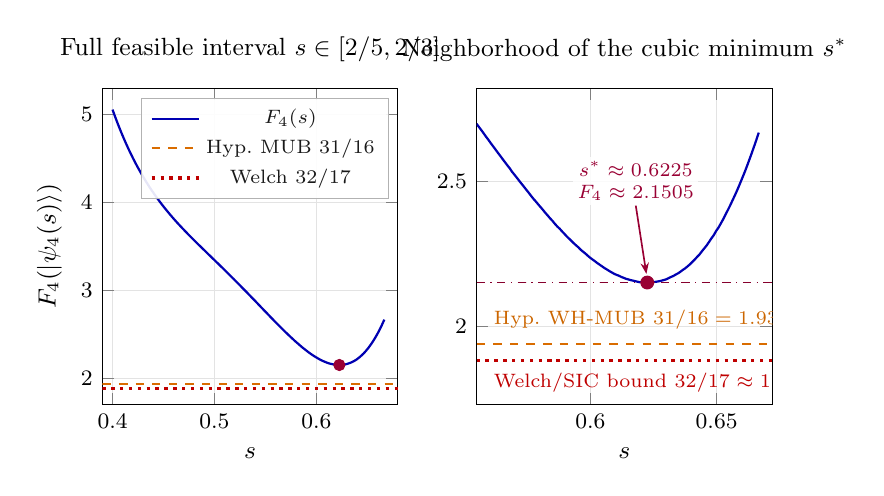
\begin{tikzpicture}
\begin{axis}[
  name=leftplot,
  width=0.44\textwidth,
  height=5.6cm,
  xlabel={$s$},
  ylabel={$F_4(\ket{\psi_4(s)})$},
  title={Full feasible interval $s \in [2/5, 2/3]$},
  title style={font=\small},
  label style={font=\small},
  tick label style={font=\footnotesize},
  xmin=0.39, xmax=0.68,
  ymin=1.70, ymax=5.30,
  grid=major,
  grid style={gray!22},
  legend pos=north east,
  legend style={font=\scriptsize, draw=black!30, fill=white, fill opacity=0.9}
]
  \addplot[domain=0.4:0.666667, samples=120, thick, blue!70!black]
    {3397.5*x^4 - 7080*x^3 + 5520*x^2 - 1920*x + 256};
  \addlegendentry{$F_4(s)$}

  \addplot[domain=0.39:0.68, dashed, orange!85!black, thick] {1.9375};
  \addlegendentry{Hyp.\ MUB $31/16$}

  \addplot[domain=0.39:0.68, dotted, red!75!black, very thick] {1.882353};
  \addlegendentry{Welch $32/17$}

  \addplot[only marks, mark=*, mark size=2pt, purple!80!black]
    coordinates {(0.622543, 2.150520)};
\end{axis}

\begin{axis}[
  at={(leftplot.east)},
  anchor=west,
  xshift=1.0cm,
  width=0.44\textwidth,
  height=5.6cm,
  xlabel={$s$},
  title={Neighborhood of the cubic minimum $s^*$},
  title style={font=\small},
  label style={font=\small},
  tick label style={font=\footnotesize},
  xmin=0.555, xmax=0.672,
  ymin=1.73, ymax=2.82,
  grid=major,
  grid style={gray!22}
]
  \addplot[domain=0.555:0.666667, samples=120, thick, blue!70!black]
    {3397.5*x^4 - 7080*x^3 + 5520*x^2 - 1920*x + 256};

  \addplot[domain=0.555:0.672, dashed, orange!85!black, thick] {1.9375};
  \addplot[domain=0.555:0.672, dotted, red!75!black, very thick] {1.882353};
  \addplot[domain=0.555:0.672, dashdotted, purple!70!black, semithick] {2.150520};

  \addplot[only marks, mark=*, mark size=2.3pt, purple!80!black]
    coordinates {(0.622543, 2.150520)};

  \node[font=\scriptsize, purple!80!black, align=center, fill=white, fill opacity=0.85, text opacity=1, inner sep=1.5pt]
    (minlbl) at (axis cs:0.618, 2.50) {$s^* \approx 0.6225$\\$F_4 \approx 2.1505$};
  \draw[-{Stealth[length=4pt]}, purple!80!black, semithick] (minlbl.south) -- (axis cs:0.6222, 2.18);

  \node[font=\scriptsize, orange!80!black, anchor=south west] at (axis cs:0.558, 1.955)
    {Hyp.\ WH-MUB $31/16 = 1.9375$};
  \node[font=\scriptsize, red!75!black, anchor=north west] at (axis cs:0.558, 1.872)
    {Welch/SIC bound $32/17 \approx 1.8824$};
\end{axis}
\end{tikzpicture}
\caption{Pauli fourth moment $F_4(\ket{\psi_4(s)})$ of the $4$-qubit spike-plus-uniform family over its feasible interval $s \in [2/5, 2/3]$ (left) and zoomed near the unique cubic minimum $s^* \approx 0.622543$ (right). For phase states, \Cref{cor:gowers} forces $F_4 > 31/16$ strictly; for general states on $\CP^{15}$, the only known analytic lower bound is the Welch/SIC bound $32/17$.}\label{fig:spike-f4}
\end{figure}

\begin{remark}[Companion numerical observation on $\CP^{15}$]\label{rem:cp15-numerics}
Separate from our Lean~4 formalization, we performed $3{,}000$ multi-start Riemannian optimizations of $F_4$ over the full $30$-real-dimensional complex projective space $\CP^{15}$. Remarkably, $2{,}936$ runs converged to the exact cubic optimum $F_4(\ket{\psi_4(s^*)}) \approx 2.1505201547$ ($M_2 \approx 2.006879$), with no state attaining a smaller value of $F_4$. Note the proper direction of comparison against the unreachable WH-MUB benchmark: $F_4(s^*) \approx 2.150520 > 31/16 = 1.9375$, equivalently $M_2(s^*) \approx 2.006879 < \ln(256/31) \approx 2.111190$. Certifying whether $F_4(\ket{\psi_4(s^*)})$ is indeed the true global minimum over all of $\CP^{15}$ remains an intriguing open problem (\Cref{op:e28-4qubit}).
\end{remark}

% ==============================================================================
\section{Pure-Kernel Formalization and Verification in Lean~4}\label{sec:lean}
% ==============================================================================

Because the even-$n$ proof relies on delicate $2$-adic divisibilities, sign-parity cancellations across affine subspaces, and an inductive M\"obius calculation, we formalized the entire proof chain in Lean~4~\cite{demoura2021lean4} atop Mathlib~\cite{mathlib2020lean}.

\subsection{Trust base and axiom audit}

The complete library \texttt{MultiQubitMUB} is pinned to Lean~4 \texttt{v4.36.0} and Mathlib \texttt{v4.36.0} and comprises $5{,}152$ lines across six core modules plus root/audit files (\Cref{tab:lean-map}). Verification satisfies strict pure-kernel hygiene:
\begin{itemize}[leftmargin=1.8em]
  \item \textbf{Zero escapes:} Automated source inspection confirms that none of \lean{sorry}, \lean{native\_decide}, custom \lean{axiom}, \lean{unsafe}, \lean{implemented\_by}, or \lean{extern} occur anywhere in the Lean source files.
  \item \textbf{Standard axioms only:} The audit script \lean{Audit.lean} runs \lean{\#print axioms} on all $10$ starred theorems in \Cref{tab:lean-map}; every theorem depends exclusively on the three standard foundational axioms of Lean~4/Mathlib: \lean{propext}, \lean{Classical.choice}, and \lean{Quot.sound}.
  \item \textbf{Numerical cross-check and CI:} The script \lean{scripts/verify\_claims.py} independently verifies the $n = 2$ witness, the antiunitary $(H^{\otimes n}\circ K)$ symmetry, the exact Pauli fourth moments for $n = 1, 2, 3, 4$, the minimal polynomial of $F_4(s^*)$, and the rational certificate $s = 622543/1000000$. Full build, axiom audit, keyword check, and Python cross-check run automatically via GitHub Actions CI.
\end{itemize}

\begin{table}[htbp]
\centering
\caption{Module structure and exact correspondence between results in this paper and machine-verified Lean~4 declarations in \texttt{MultiQubitMUB} (total $5{,}152$ lines including \texttt{MultiQubitMUB.lean} and \texttt{Audit.lean}). Asterisks~($^*$) mark the $10$ headline theorems audited in \texttt{Audit.lean}.}\label{tab:lean-map}
\smallskip
\footnotesize
\setlength{\tabcolsep}{4pt}
\renewcommand{\arraystretch}{1.22}
\begin{tabular}{@{}l r >{\raggedright\arraybackslash}p{3.6cm} >{\raggedright\arraybackslash}p{6.6cm}@{}}
\toprule
Lean module & Lines & Paper result & Key Lean declarations ($^*$ = audited) \\
\midrule
\leantab{GaussianInt.lean} & 280 & Lemmas~\ref{lem:sq-descent}, \ref{lem:gi-pi-descent} &
  \leantab{sq\_add\_sq\_eq\_pow\_two\_even}, \leantab{sq\_add\_sq\_eq\_pow\_two\_odd}, \leantab{pow\_giPi\_dvd\_of\_pow\_two\_dvd\_norm} \\
\leantab{Basic.lean} & 364 & Lemma~\ref{lem:wht} &
  \leantab{wht\_inversion}, \leantab{sum\_chi\_affine}, \leantab{even\_card\_dot\_one}, \leantab{odd\_card\_nonzero\_dot\_zero} \\
\leantab{SubspaceInduction.lean} & 1{,}072 & Lemmas~\ref{lem:mobius}--\ref{lem:prod-diff}, Thm.~\ref{thm:subspace-induction}, Lem.~\ref{lem:wht-subcube} &
  \leantab{mobius\_inversion}, \leantab{subspaceVal\_of\_corrCongr}, \leantab{pow\_two\_dvd\_wht\_sub\_of\_subspaceVal} \\
\leantab{Alltop.lean} & 1{,}273 & Theorem~\ref{thm:no-alltop}, Corollary~\ref{cor:gowers} &
  \leantab{no\_alltop\_f2}$^*$, \leantab{exists\_alltop\_two}$^*$, \leantab{phasePauliMoment4\_gt\_mub}$^*$ \\
\leantab{PauliGroup.lean} & 1{,}725 & Theorems~\ref{thm:no-pauli-mub}, \ref{thm:odd-two-valued}, Cor.~\ref{cor:damski-lly}, Prop.~\ref{prop:sharpness}(i) &
  \leantab{no\_pauli\_mub\_fiducial}$^*$, \leantab{damski\_conjecture\_1}$^*$, \leantab{no\_pauli\_two\_valued\_odd}$^*$, \leantab{exists\_pauli\_mub\_fiducial\_two}$^*$ \\
\leantab{SpikeFamily.lean} & 413 & Theorem~\ref{thm:spike} &
  \leantab{pauliMoment4\_spikeState}$^*$, \leantab{hoggar\_sic\_three}$^*$, \leantab{four\_qubit\_spike\_bound}$^*$ \\
\bottomrule
\end{tabular}
\end{table}

\subsection{Architectural design choices and specification fidelity}

Three deliberate mathematical design choices kept the formalization compact, fast, and transparent:
\begin{enumerate}[leftmargin=1.8em]
  \item \textbf{Zero-UFD Gaussian integer arithmetic (\lean{GaussianInt.lean}):} Instead of invoking Mathlib's unique-factorization or principal-ideal-domain machinery for $\Zi$, both \Cref{lem:sq-descent} and \Cref{lem:gi-pi-descent} are proved by elementary integer descent in $280$ lines.
  \item \textbf{Completely matrix-free quantum mechanics (\lean{PauliGroup.lean}):} Representing $n$-qubit states directly as functions \lean{QState n := F2 n -> Complex} avoids $2^n \times 2^n$ complex matrix algebra, Kronecker-product reindexing, and spectral-theorem overhead. Pauli completeness, symplectic self-duality, purity, the explicit symplectic basis (\Cref{lem:symp-basis}), and the trace-certified joint $+1$ eigenstate (\Cref{lem:mub-to-alltop}) are all established directly on function spaces.
  \item \textbf{First-principles specifications:} The predicates \lean{IsAlltop} and \lean{IsPauliMubFiducial} encode \Cref{def:alltop,def:pauli-mub} directly with no hidden regularity assumptions; equal fiber sizes and equimodularity are proved inside \lean{no\_pauli\_mub\_fiducial}. All $10$ audited theorems reside at the top level of \lean{MultiQubitMUB} and can be checked via \lean{lake build \&\& lake env lean Audit.lean}.
\end{enumerate}

% ==============================================================================
\section{Discussion and Open Problems}\label{sec:open}
% ==============================================================================

Our theorems close the existence question for complete $2^n$-basis multi-qubit Pauli-covariant MUB fiducials and Alltop functions on $\F_2^n$, while opening several concrete quantitative and structural problems.

\begin{openproblem}[Quantitative Gowers $U^3$ gap on $\F_2^n$]\label{op:gowers-gap}
By \Cref{cor:gowers} and compactness of the $2^n$-torus $\Uone^{\F_2^n}$, the minimum over all unimodular functions strictly exceeds $2 - 2^{-n}$ for every $n \ge 3$. What is the asymptotic behavior of the optimal excess
\[
  \Delta_{\mathrm{phase}}(n) := \min_{\phi : \F_2^n \to \Uone} 2^n \norm{\phi}_{U^3(\F_2^n)}^8 - (2 - 2^{-n})
\]
as $n \to \infty$? Does $\Delta_{\mathrm{phase}}(n)$ decay exponentially in $n$, or remain bounded away from zero (or even grow)?
\end{openproblem}

\begin{openproblem}[Four-qubit maximal magic / Open Quantum Problem~E28]\label{op:e28-4qubit}
Prove (or refute) that the cubic spike-plus-uniform state $\ket{\psi_4(s^*)}$ of \Cref{thm:spike} globally minimizes $F_4(\ket{\psi})$ over all pure states $\ket{\psi} \in \CP^{15}$, i.e., that
\[
  \min_{\ket{\psi} \in \CP^{15}} F_4(\ket{\psi}) = F_4(\ket{\psi_4(s^*)}) \approx 2.1505201547.
\]
Even a weaker analytic lower bound strictly beating the Welch/SIC bound $32/17 \approx 1.882353$ (or beating the unreachable WH-MUB benchmark $31/16 = 1.9375$) for \emph{general} non-equimodular states in $\CP^{15}$ would represent a major advance on Problem~E28~\cite{oqpE28}.
\end{openproblem}

\begin{openproblem}[Maximum partial sets of Pauli-covariant MUBs]\label{op:partial-mub}
\Cref{thm:no-pauli-mub} rules out a single fiducial generating $2^n$ pairwise MUBs under $\Pauli_n$ for $n \ge 3$. What is the maximum number $k_{\max}(n) < 2^n$ of pairwise mutually unbiased orthonormal bases that can be realized as a subset of a single Pauli orbit $\{P_p\ket{\psi}\}_{p \in \F_2^{2n}}$ for $n \ge 3$?
\end{openproblem}

\begin{openproblem}[Higher-$n$ extremal magic beyond the spike family]\label{op:higher-n}
For $n = 5$, numerical minimization of \eqref{eq:spike-poly} over the feasible interval $[0.4249, 0.6074]$ yields $F_5 \approx 3.300037$ ($M_2 \approx 2.271802$), well above $2 - 2^{-5} = 1.96875$. Understanding whether higher-$n$ maximal magic states continue to exhibit large finite symmetry groups (such as $\GL(n,\F_2)$ or symplectic subgroups of the Clifford group) or transition to less symmetric configurations remains wide open.
\end{openproblem}

\bibliographystyle{plainurl}
\bibliography{references}

\end{document}
